\documentclass[landscape,letter]{article}
\usepackage[fontsize=11pt]{scrextend}
\usepackage[utf8]{inputenc}
\usepackage[ngerman]{babel}
\usepackage[dvipsnames]{xcolor}
\usepackage{tikz}
\usetikzlibrary{shapes,positioning,arrows,fit,calc,graphs,graphs.standard}
\usepackage[nosf]{kpfonts}
\usepackage[t1]{sourcesanspro}
%\usepackage[lf]{MyriadPro}
%\usepackage[lf,minionint]{MinionPro}
\usepackage{multicol}
\usepackage{wrapfig}
\usepackage[top=0mm,bottom=1mm,left=0mm,right=1mm]{geometry}
\usepackage[framemethod=tikz]{mdframed}
\usepackage{microtype}
\usepackage{listings}
\usepackage{bussproofs}
\EnableBpAbbreviations

\let\bar\overline

\definecolor{myblue}{cmyk}{1,.72,0,.38}

\def\firstcircle{(0,0) circle (1.5cm)}
\def\secondcircle{(0:2cm) circle (1.5cm)}

\colorlet{circle edge}{myblue}
\colorlet{circle area}{myblue!5}
\definecolor{rred}{HTML}{b61010}
\tikzset{filled/.style={fill=circle area, draw=circle edge, thick},
    outline/.style={draw=circle edge, thick}}

\pgfdeclarelayer{background}
\pgfsetlayers{background,main}

\renewcommand{\baselinestretch}{.8}
\pagestyle{empty}

\global\mdfdefinestyle{header}{%
linecolor=gray,linewidth=1pt,%
leftmargin=0mm,rightmargin=0mm,skipbelow=0mm,skipabove=0mm,
}

\newcommand{\header}{
	\mdfsetup{%
		middlelinecolor=black,
		middlelinewidth=2pt,
                backgroundcolor={rred},
		%roundcorner=10pt}
	}
\begin{mdframed}[style=header]
\footnotesize
\sffamily
%\colorbox{yellow}

{COMP 527 Crib Sheet}\\
by~{Julian Lore}~Side \thepage \ of 2
\end{mdframed}
}

\makeatletter
\renewcommand{\section}{\@startsection{section}{1}{0mm}%
                                {.2ex}%
                                {.2ex}%x
                                {\sffamily\small\bfseries}}
\renewcommand{\subsection}{\@startsection{subsection}{1}{0mm}%
                                {.2ex}%
                                {.2ex}%x
                                {\sffamily\bfseries}}



\def\multi@column@out{%
   \ifnum\outputpenalty <-\@M
   \speci@ls \else
   \ifvoid\colbreak@box\else
     \mult@info\@ne{Re-adding forced
               break(s) for splitting}%
     \setbox\@cclv\vbox{%
        \unvbox\colbreak@box
        \penalty-\@Mv\unvbox\@cclv}%
   \fi
   \splittopskip\topskip
   \splitmaxdepth\maxdepth
   \dimen@\@colroom
   \divide\skip\footins\col@number
   \ifvoid\footins \else
      \leave@mult@footins
   \fi
   \let\ifshr@kingsaved\ifshr@king
   \ifvbox \@kludgeins
     \advance \dimen@ -\ht\@kludgeins
     \ifdim \wd\@kludgeins>\z@
        \shr@nkingtrue
     \fi
   \fi
   \process@cols\mult@gfirstbox{%
%%%%% START CHANGE
\ifnum\count@=\numexpr\mult@rightbox+2\relax
          \setbox\count@\vsplit\@cclv to \dimexpr \dimen@-1cm\relax
\setbox\count@\vbox to \dimen@{\vbox to 1cm{\header}\unvbox\count@\vss}%
\else
      \setbox\count@\vsplit\@cclv to \dimen@
\fi
%%%%% END CHANGE
            \set@keptmarks
            \setbox\count@
                 \vbox to\dimen@
                  {\unvbox\count@
                   \remove@discardable@items
                   \ifshr@nking\vfill\fi}%
           }%
   \setbox\mult@rightbox
       \vsplit\@cclv to\dimen@
   \set@keptmarks
   \setbox\mult@rightbox\vbox to\dimen@
          {\unvbox\mult@rightbox
           \remove@discardable@items
           \ifshr@nking\vfill\fi}%
   \let\ifshr@king\ifshr@kingsaved
   \ifvoid\@cclv \else
       \unvbox\@cclv
       \ifnum\outputpenalty=\@M
       \else
          \penalty\outputpenalty
       \fi
       \ifvoid\footins\else
         \PackageWarning{multicol}%
          {I moved some lines to
           the next page.\MessageBreak
           Footnotes on page
           \thepage\space might be wrong}%
       \fi
       \ifnum \c@tracingmulticols>\thr@@
                    \hrule\allowbreak \fi
   \fi
   \ifx\@empty\kept@firstmark
      \let\firstmark\kept@topmark
      \let\botmark\kept@topmark
   \else
      \let\firstmark\kept@firstmark
      \let\botmark\kept@botmark
   \fi
   \let\topmark\kept@topmark
   \mult@info\tw@
        {Use kept top mark:\MessageBreak
          \meaning\kept@topmark
         \MessageBreak
         Use kept first mark:\MessageBreak
          \meaning\kept@firstmark
        \MessageBreak
         Use kept bot mark:\MessageBreak
          \meaning\kept@botmark
        \MessageBreak
         Produce first mark:\MessageBreak
          \meaning\firstmark
        \MessageBreak
        Produce bot mark:\MessageBreak
          \meaning\botmark
         \@gobbletwo}%
   \setbox\@cclv\vbox{\unvbox\partial@page
                      \page@sofar}%
   \@makecol\@outputpage
     \global\let\kept@topmark\botmark
     \global\let\kept@firstmark\@empty
     \global\let\kept@botmark\@empty
     \mult@info\tw@
        {(Re)Init top mark:\MessageBreak
         \meaning\kept@topmark
         \@gobbletwo}%
   \global\@colroom\@colht
   \global \@mparbottom \z@
   \process@deferreds
   \@whilesw\if@fcolmade\fi{\@outputpage
      \global\@colroom\@colht
      \process@deferreds}%
   \mult@info\@ne
     {Colroom:\MessageBreak
      \the\@colht\space
              after float space removed
              = \the\@colroom \@gobble}%
    \set@mult@vsize \global
  \fi}

\makeatother
\setlength{\parindent}{0pt}

\begin{document}
\small
\begin{multicols*}{5}
  \color[HTML]{11114E}
\section{Uninformed Search}
\paragraph{Search Problem} \textbf{State space} $S$: all possible configs of
domain, \textbf{init state} $s_0 \in S$, \textbf{goal
states} $G \subset S$ (end states), \textbf{Operators} $A$ (actions
avail), \textbf{Path}, \textbf{Path cost}, $c$, \textbf{Soln} path
$s_0 \to s_g\in G$, \textbf{Opt
  soln}: path with min \$
\\ Eight puzzle: States (conf of puzzle), goals (target conf), ops
(swap blank with adj), path cost (\# moves)
% \\ Basic assumptions for now: (static, observable, deterministic env,
% discrete states)
\\ Rep state space search as graph, verts are states, edges
are ops. Build \textbf{search tree} to find goal
state. \underline{Search tree nodes not same as graph nodes}
\\ Data struct for search tree: \textbf{Node} (state id, parent state
+ op, cost of path, depth. To expand node, apply all legal ops and gen
new nodes.
\paragraph{Generic search alg} Init search tree with $s_0$. Loop: If
no nodes can be expanded, fail. Else choose node to expand, if node
has goal, return path, else expand node by applying each op and
getting new states, adding to tree.
\paragraph{Uninformed (blind) search} If state isn't goal, you
\colorbox{red}{don't
know how close} to goal it might be.
\paragraph{Uninformed Search algs}
\colorbox{yellow}{Key props}:  \textbf{Completeness} (guarantee soln if it exists),
\textbf{Optimality} (how good is soln), \textbf{space complexity},
\textbf{time complexity}.
\subparagraph{Search complexity} \textbf{Branching factor} $b$,
\textbf{solution depth} $d$
\\ All uninf search time complex $O(b^d)$, very general and very
expensive, no knowledge.
\\ \textbf{Breadth-first search} (\colorbox{yellow}{complete} w/ finite $b$, guaranteed
shortest path if unit cost = \colorbox{yellow}{optimal}, but not if
weighted graph). \colorbox{yellow}{$O(b^d)$} space. \textbf{depth-first
  search} (\colorbox{yellow}{$O(bm)$} space, easy to do recursively, more efficient than
BFS if many goal paths, \colorbox{yellow}{\textbf{not optimal}}, may not complete
(cycles), don't use DFS for big $d$), \textbf{uniform-cost search}
(BFS but with \textbf{general} (weighted graph) step costs, use a
pqueue, \colorbox{yellow}{opt \& comp}), \textbf{depth-limited search} (DFS but stop at goal or max
depth, always terms, but \colorbox{red}{not complete}),
\textbf{iterative deepening search}(depth-lim search but increasing
depth, expands nodes mult times, \colorbox{yellow}{complete}, \colorbox{yellow}{linear mem req} like DFS,
but more time, \colorbox{yellow}{optimal} if unit cost, preferred for large state spaces)
\\ Revisiting states: maintain \textbf{closed list} to store expanded
nodes, good for probs with repeated states. $O(|S|)$ time and
space. Sometimes re-expanding states could be better (compare old and
new path cost, also sometimes domain may be too large to store all
states).
\\ \colorbox{yellow}{What method to use?} To find opt: BFS, IDS for unit cost,
uniform-cost search if general cost. Large state space: DFS max length
is known, IDS otherwise. Limited mem: DFS/IDS. Quickly find best soln
with budget: Depth-limited if unit cost, UCS if gen cost.
\color{Orange}
\section{\textcolor{Orange}{Informed Search}} Use \textbf{heuristics} to guide search. Uninformed
expand nodes based on dist from start node. Informed expands based on
\textbf{distance to goal}. If we don't know exact distance, we use
intuition, \textbf{heuristic}. Heuristics come from prior knowledge of
prob, exact soln to \colorbox{yellow}{relaxed vers} of prob, learning from exp
\\ Heuristic for path planning: straight-line distance between two places.
\\ Eight puzzle: number of misplaced tiles, total Manhattan dist
\paragraph{Algs} \textbf{Best-First Search}(\colorbox{yellow}{greedy}, expand most
promising node first, close to BFS, if heuristic is 0, then same as
BFS, opp of UCS(cost-so-far) vs cost-to-go, $O(b^d)$ time/space, good
heuristic can make $O(bd)$, \textbf{not always complete}(loops), but
complete if finite space if we check repeated, \colorbox{red}{not optimal}), \textbf{Heuristic
  Search}(Problem: best-first 
too greedy, doesn't account for cost so far. Soln: \textbf{Heuristic
  search}, greedy wrt to $f = g+h$, $g$ is cost so far, $h$ is
heur. Use pq, add to q w/ p: $f = g + h$, end when goal popped
from q. Note we cont expanding nodes after finding goal if
$\exists$ unexpanded w/ lower cost than current path to goal. \colorbox{red}{Not
optimal}, unless we put conds on heuristics),
\textbf{A* Search} (Heuristic search with AH. \colorbox{green}{Complete},
$f(s)=g(s)+h(s)\leq g(s)+c(s,s')+h(s')=f(s')$ by consistency, so no
node can be re-expanded. If soln, c must b bounded, so $A*$ will
find. \colorbox{green}{Opt}, prove by contradiction, showing impossible that subopt
goal is expanded before opt. Still worst case $O(b^d)$, but $O(bd)$
with perfect heuristic because only expand nodes on opt path. With
given $h$, no other search alg can expand less nodes),
\textbf{Iterative Deepening A*}(DFS, but use $f$ to determine order to
explore children. Stop at $f$ val instead of d. Same props as $A*$, but less
mem. If we remember expansion of old nodes $\to$ SMA*)
\paragraph{Admissible heuristics} $h^*(n)$ is shortest p from $n$ to
any goal. $h$ is \textbf{admissible heuristic} if $h(n) \leq h^*(n)
\forall n$. They are optimistic. Trivial ah: $h(n)=0 \forall n$, get
UCS. Obviously $h(g)=0 \forall g \in G$ for AH. Usually relaxed vers
of prob gives AH.
\paragraph{Consistency} AH $h$ is called \textbf{consistent/monotone*}
if for every state $s$ and succ $s'$, $h(s) \leq c(s,s') + h(s')$,
i.e. $h$ gets more precise as we get closer to goal. Vers of triangle
ineq. Can fix inconsistent heuristics by: $f(s')=g(s')+h(s') \to
f(s')=\max\{g(s')+h(s'),f(s)\}$
\paragraph{Dominance} $h_2(n) \geq h_1(n) \forall n$ and both AH, then
$h_2$ dominates $h_1$, i.e. more informative.
\paragraph{Decomposition} Break complex prob into smaller
parts. Decomp and putting soln together may give up optimality. Use
decomp for probs we can't solve w/o. Subsolns can be cached \&
reused. Need to be careful that when we chose subgoal, overall prob
still has soln. \textbf{Macro-action} is sequence of actions from orig problem
(e.g. make T for Rubik's)
\\ \textbf{Abstraction} ignores info to speed up comp, make compact
representation, map several real states to one abstract state
\\ Consistency stronger than admissibility, cannot be cons but not
admis. A$^*$ space vs ID depends on how good heur is. DFS is special
case of best-first.
\color[HTML]{008080}
\section{\textcolor[HTML]{008080}{Optimization}}
large cont/combin state space. Can't search all
possible soln. Non-uniform cost.
\paragraph{Traveling salesman prob} Vertices+dist between pairs. Get
shortest path to visit each vert once. Tour = path that satisfies
goal.
\\ Optimization prob described by \textbf{states} and
\textbf{evaluation function}, note that states are candidate solutions
(can be partial or wrong)
here, \colorbox{red}{not descrp of world}. Func corresp to
path cost.
\paragraph{Optimization Search}
\textbf{Constructive methods}, start from scratch, build
up. \textbf{Iterative improvement}, start with soln, improve. Both
involve \colorbox{green}{local} search.
\paragraph{Generic local search}
Start at init $X_0$, repeat until satisfied: Gen neighbors of $X_i$;
eval them. Select 1 neighbor $X_{i+1}$ to become current
config.
\paragraph{Discrete Hill-Climbing}Start with $X_0$, val
$E(X_0)$. Repeat until sat: Gen
neighbors of $X$ and $E(X_i)$. Get $\max_i E(X_i)$. If max is
less than $E_{\max x}$ of init, then return. Else update $X$ to be new $X_i$
and $E$ to be new $E_{\max}$. This is a variant of best-first search,
easy to prog, no memory of past req, can handle large probs. Small
neighborhood = less neighbors, possibly worse soln, large
neighborhood = more to eval, possibly less local optima, better
soln. \colorbox{red}{Problem:} hill climbing can easily get stuck in
plateau or local opt, to fix, use random re-starts or pick any move
that leads to improvement (\textbf{randomize hill climbing}).
\paragraph{Simulated annealing} Like hill climbing, but allows bad
moves to escape local opt. Decrease size+freq of bad moves over
time. \\Alg: Start with $X_0$ and $E(X_0)$. Loop until satisfied:
choose random neighbor, if val is greater than $E_{max}$, replace
current max. If greater than current val we holding, replace current
$X$. Else, with prob $p$, still replace cur val. Return max at end.
\\ What to use for $p$? Constant, val that decays to $0$, val that
depends on how bad move is. We usually use \colorbox{green}{Boltzmann
  distribution}$\mathbf{p = e^{-(E-E_i)/T}}$, bad $E_i \to $small
$p$. T here is called \textbf{temperature}, usually start high then
decrease to 0 over time. Can decrease $T$ by mult by constant $0 <
\alpha < 1$ at every iter. If T is high $\to$ alg is in exploratory
phase, if low, exploitation phase.
\\ If T decreases ``slowly enough'', \colorbox{green}{optimal}, but
may take $\infty$ moves. SA better than HC when lots of local opt. HC
preferred if func is smooth, not many local opt, most local opt are
similar.
\paragraph{Parallel search} Run mult separate searches (HC or SA) in
parallel, keep best soln
\paragraph{Local beam search} Like parallel search, but share info
across searches. Start $k$ searches in parallel, but keep $k$
(\textbf{beam width}) top
solns at each step.
\paragraph{Genetic algs} \textbf{Individual}=candidate soln. Each
indiv has \textbf{fitness} (quality of soln). \textbf{Population} =
set of indivs. Pops change over \textbf{generations} by applying
\textbf{operations}(mutation(inject random change with mutation rate =
prob of mutation occur)/crossover(combine parts of indivs to make new
indiv, use \textbf{crossover mask} to specify which parts taken from 1
indiv as bin string, rest taken from other)/selection) to indivs. Higher
fitness = more likely to survive \& reproduce. Usually represent
indivs by \textbf{binary string}.
\\ \colorbox{yellow}{Alg}: (params: fitness,threshold,p,r,m) \underline{init} $P$ with
$p$ rand indivs. \underline{Eval}, get Fitness(h) $\forall h \in
P$. While $\max_h Fitness(h)<threshold$: Select $(1-r)p$ members of
$P$ to put in $P_s$. Crossover $\frac{rp}{2}$ pairs of indivs. For
each pair, produce two offspring and incl in $P_s$. Mutate 1 rand bit
in $mp$ rand indivs of $P_s$. Update $P \gets P_s$. Eval fitness
$\forall h \in P$. After loop return ind w/ max fit.
\paragraph{Selection} Survival of fittest: \textbf{Fitness
  proportionate}, might lead to crowding (mult copies of same soln),
\textbf{tournament selection}, pick 2 rand indivs, with prob $p$
select fitter one. \textbf{Rank selection}, sort all by fitness, prob
of selection proportional to rank. \textbf{Softmax (Boltzman)
  selection}
$P(i)=\frac{e^{Fitness(i)/T}}{\sum_{j=1}^{P}e^{Fitness(j)/T}}$.
\\ \colorbox{yellow}{Elitism}, best soln can die during evol, so we
preserve best soln encountered. Genetic algs more expensive than HC \&
SA.
\paragraph{Pros cons of gen alg} \colorbox{green}{Pro:} Intuitive due to analogy, can be
effective if tuned properly. \colorbox{red}{Bad:} Perform dependent on
encoding of problem. Many params to tweak. Low mutation rate =
overcrowding. Too high = too random.
\\ Search ops: mutation, xover, select
\color[HTML]{A10F6F}
\section{Constraint Satisfaction Problems} Use constraints to
\colorbox{green}{narrow} search space. Def: \textbf{variables} $V_i$
that can take vals from domain $D_i$. \textbf{Constraints} specifying
allowed combinations of values for variables. Constraints can be
represented as a function or list of allowable vals. \textbf{CSP
  solution} is assignment of vals to vars st all constraints
true. Usually want to find \underline{any soln} or find that no soln
exists.
\paragraph{Approaches}
\textbf{Constructive approach}, state = vals assigned so far. Use
\colorbox{green}{forward search} to fill soln. Gen purpose, works for
all CSPs. \textbf{Random approach}, start with broken complete assn of
vals to vars. Fix broken constrs by re-assign vars. Use optimization.
\paragraph{Problem def}\textbf{State} (vals assigned so far, can be
partial/inconsistent). \textbf{Initial state} (all vars
unassgn). \textbf{Operators} (assign val to unass var). \textbf{Goal
  test} = all vars assigned, no constraint false, complete and
consistent assignment. Problem is
\colorbox{green}{deterministic}. Note that \colorbox{yellow}{depth is
  limited to \# of vars}, can use DFS or depth-limited search.
\\ Uninformed search for map coloring: choose unassigned var, assign a
val. This is complete and optimal, but complexity is worst possible,
$n! d^n$, ($n$ vars, $d$ vals). Branching factor \colorbox{red}{very
  high}. Var assgnment order irrelevant, many paths equiv.
\paragraph{Constraint graph}Nodes are vars, \colorbox{green}{arcs}
show constraints. Can use graph struct to accelerate search. Use
\textbf{inference} to reduce search
space. \colorbox{green}{pre-process} graph to remove
inconsistencies. Var is \textbf{arc-consistent} if all val in domain
satisfies vars binary constraints. Network is \textbf{generalized
  arc-consistent} if all vals in domain of all vars are all
arc-cons. \colorbox{yellow}{Keep applying arc-consistency} until no
changes to get generalized arc-cons.
\paragraph{Ex} Map coloring: vars = countries, domains = r,g,b,
constraints = adj countries cannot be same color, $C_1 \neq C_2
\ldots$.
\\ 4 queens: 1 queen/col, vars = $Q_1, \ldots$, row of each
queen. Domain = ${1,2,3,4}$. Constraints: $Q_i \neq Q_j$ (not same
row), $|Q_i-Q_j| \neq |i-j|$ (not same diag)
\paragraph{Backtracking search} DFS but fix order of var assn $b =
|D_i|$. If no assignment for specific var, backtrack to prev var and
try diff val. Basic uninformed alg.
\paragraph{Forward checking} Keep track of legal vals for unassigned
vars. When you assign vars, look at unassigned vars connected via
constraint and delete from their domain any inconsistent vals to new
assgn.
\paragraph{Heuristics for CSP} For selecting vars:
\textbf{minimum-remaining vals} = choose var that is most
constrained (least remain vals) \colorbox{green}{more info} if one branch is not
satisfiable ($1/2$ of branches bad vs $1/100$ branches bad). \textbf{Degree heuristic} = choose var that imposes most
constraints on remaining vars, can use to break ties from min-remain
vals heuristic. To select a val: \textbf{least-constraining val}:
assign a val that rules out fewest vals for other vars
(\colorbox{green}{less chance of conflict} in future).
\\ Worst-case $d^n$. $d$ \# vals, $n$ \# vars. Tree structured constraint graph gives
$O(nd^2)$. Nearly-tree structured: $O(d^c(n-c)d^2)$ using
\textbf{cutset conditioning}, find vars st removing them turns graph
into tree. Instantiate them all possible ways, $c$ is size of cutset.
\paragraph{Local search} \textbf{Iterative improvement alg} Start with
broken but complete assnment of vals \& vars. Allow var assgns that
don't satisfy some constraints. Randomly select conflicted vars. Ops
reassign var vals. \textbf{min-conflict heuristic} chooses val that
violates fewest constraints. This is hill climbing.
\color[HTML]{8b0000}
\section{Uncertainty} Actions may be
\textbf{non-deterministic} or det. Problems can be \textbf{(fully) observable},
\textbf{partially observable}(det or nondet) or \textbf{non-observable}.
\paragraph{Searching under uncert} Cannot determine future states in
advance (i.e. depend on die roll). Soln is not path, but
\textbf{contingency plan/strategy}.
\\ Vacumm ex. Two rooms, vacuum in one of the rooms, rooms can be
dirty or clean. When non-observable, need plan. What states possible
after doing an action? Reason over \textbf{beliefs} (sets of
states). \colorbox{green}{Total \# possible beliefs} = power set of
all states w/o empty. Less \colorbox{yellow}{reachable beliefs}
though.
\paragraph{Conformant planning} Find plan that leads to goal
\colorbox{green}{despite state uncertainty}. Good heur, use acts
that red uncertainty, red belief to 1 state, then do standard
search.
\\ \textbf{Non-deterministic} case: vacuum may sometimes deposit dirt
instead of cleaning, sweep may sometimes clean adjacent. Make
\textbf{AND-OR} search tree: \textbf{OR nodes} (agent chooses between
actions), \textbf{AND nodes} (choice induced by env choice of outcome,
non-det). Want subtree st \colorbox{green}{all leaves are goal
  leaves}. Soln is subtree that specifies one act at each OR node,
inclds every outcome at each AND node, has goal node at ea leaf.
\\ Slippery vacuum, moving sometimes fails. Apply \textbf{cyclic}
soln, keep trying until it works. Can be ok soln if caused by
\colorbox{green}{random event} but not if caused by unobserved event,
like \colorbox{red}{broken} vacuum, can't move.
\paragraph{Partial observability} Can only sense things locally,
i.e. if current room is dirty. Account for possible observations that
tell us about next state. Search over belief
states. \colorbox{red}{Problems} \# of reachable beliefs can be v
large (use sampling or pruning). \# of states in each belief can b
v large (use compact state rep, plan for each state sep)
\\ Mastermind: belief space: pow set of all colors. Init belief set of
possible col. Act space: choosing col combo. Det: code doesn't change,
non-det: don't know percepts. Percepts: white/red pegs. Goal test: 4
reds, step cost $\frac{1}{\# \ tries}$
\color[HTML]{8A2BE2}
\section{Game Playing} We have \textbf{perfect} vs
\textbf{imperfect}(hidden info) info, and \textbf{deterministic} vs
\textbf{stochastic} (chance) games.
\paragraph{Game playing as search} 2-player, perfect, determ
games. State: state of board/player turn, ops: legal moves, goal:
states st W/L/D, cost: basic ($+1, 0, -1 \to $W/D/L), complex (points
won, money, \ldots). \colorbox{green}{Want strat(way of picking moves)
  to max utility(prob of win/min cost)}. We assume adversary is trying
to minimize \& playing optimally, \colorbox{red}{Bad assumption}.
\\ Define \textbf{max player} (wants to max util) \& \textbf{min
  player} (to min util).
\paragraph{Minimax search} Expand complete search tree until terminal
states have been reached, compute util. Go back up from leaves towards
cur state. At \textbf{min nodes}, backup worst val of children, at \textbf{max nodes},
backup best val, where min/max nodes correspond to min/max
players. \colorbox{green}{Complete} (if tree finite),
\colorbox{green}{optimal} if advers playing opt, $O(b^m)$ time,
$O(bm)$ space if DFS. \colorbox{red}{Issues} v expensive even w/
pruning. Req reasonable eval func. Assum both players playing
opt wrt same eval func. What if non-determinism in game or don't know
game well enough to make good eval func? $\to$ \textbf{random sims}.
\paragraph{\colorbox{red}{Resource limitations}} Might be time
restricted, can't search all nodes. Can use cutoff test (based on
depth) \& eval func ($v(s)$ represents ``goodness'' of board state,
chance of winning at that pos. If features of board can be eval indep,
use weighted linear func) for nodes @ cutoff. \textbf{Real-time
  search}. Eval func for chess can be \# white queens $-$ \# black
queens + \# white pawns $-$ \# black pawns \ldots. Move chosen should
be same if we apply monotonic trans to eval func. Minimax cutoff: stop
at some max depth, use eval func.
\paragraph{$\alpha\hbox{-}\beta$ pruning} If path looks worse than
what we have, discard. If best move at node \colorbox{yellow}{cannot change}, \colorbox{red}{don't
search further}. Minimax but keeps track of best leaf val for player
($\alpha$) and opponent ($\beta$), gives bounds
$[\alpha,\beta]=[-\infty,\infty]$ at start. Update $\alpha$ at max and
$\beta$ at min. Pass vals up to parents as min/max, parents copy their
bounds to children. \colorbox{green}{Pruning can greatly incr
  eff}. Pruning does not affect final result, best moves are
\colorbox{yellow}{same as mimimax}, assuming opponent is optimal and
eval func is good. With bad ordering, $O(b^m)$, nothing
pruned. Perfect ordering: $O(b^{\frac{m}{2}})$. Usually
$O(b^{\frac{3m}{4}})$ \colorbox{red}{Cons}, big $b$ means depth is
still too limited. Optimal only if opp is optimal. If using
heuristics, opponent needs to use same heuristic.
\paragraph{Forward pruning} (for domains with large $b$) only explore
$n$ best moves for our state. May lead to \colorbox{red}{sub-optimal}
soln. Can b v eff.
\paragraph{Strats} Make compact state rep. Using IDS for
real-time. Use $\alpha$-$\beta$ pruning w/ eval func. Searching deeper
usually more important than having good eval func. Consider diff
strats for begin, mid, end. Use rand to break ties. Consider non opt opp.
\paragraph{Random Simulations} Sim games by rand selecting moves for
both players. At end, check if won or lost, keep track of initial
move. After lots of sims, pick move w/ highest win rate. Using rand to
gen sample for estimation called \textbf{Monte Carlo method}. Spend more search effort at \textbf{promising
  moves}. Can use minimax style search for few moves at top.
\paragraph{Monte Carlo Tree Search} Search tree + Monte Carlo
sims. Select promising node in search tree using \textbf{tree policy}
(mapping from states to acts). Sample possible continuations from
leaves using rand \textbf{default policy} for both players (usually @
end of gm). Val of move = \textbf{avg of evals} from sampled
lines. Pick move with \colorbox{green}{best avg/expected val}.
\\ Alg: Init search tree with curr state of gm. Repeat until no more
comp budget: \textbf{Descent}: Choose + expand node in curr tree, use minimax
or which 1 seems more promising. \textbf{Rollout}: when @ leaf, use
MC sim to end of game/affordable d. \textbf{Update}: update stats for
all nodes visited during descent by backpropagating. \textbf{Growth}:
First state in rollout added to tree and stats initialized.
\colorbox{green}{Advantages vs $\alpha\hbox{-}\beta$} Not as
pessimistic, converges to minimax soln in limit. Perf increases w/ \#
lines of play. Unaffected by $b$. Easy to
parallelize. \colorbox{red}{Disadvantages} May miss opt play, policy
is very important.
\paragraph{Tree Policy} How to select next move in search tree?
Balance \textbf{exploitation} (node that seems promising acc to
estimates \& sims) \& \textbf{exploration} (node hasn't received many
sims, so want \textbf{more info}). Def: $Q(s,a)$: val of taking act
$a$ from state $s$. Win rate of node based on sims so far. $n(s,a)$
\# tries taken act a from state s. $n(s)$ \# times visited $s$.
\paragraph{Upper Confidence Trees}
$Q^{\oplus}(s,a)=Q(s,a)+c\sqrt{\frac{\log n(s)}{n(s,a)}}$, $c$ is
scaling constant. $1^{st}$ term is upper bound on val of taking a in
s.  $1^{st}$ term after eq is exploitation, last term is exploration
(gets smaller the more you select it). To \colorbox{green}{decide
  which action} to take, calc upper bd of all children, select
min/max.
\\ Can incr calc avg, $V_{k+1}\sum_{i=1}^{k+1}R_i = \frac{k}{k+1}V_{k}+\frac{R_{k+1}}{k+1}$
\paragraph{Rapid Action-Value Estimate} Assume val of move is same no
matter when played. Introduces bias, but reduces variability in MC
estimates. Since \colorbox{green}{only the move itself matters}, state
space is simplified, requires less sims (don't need many sims for each
indiv pos), but might \colorbox{red}{oversimplify} board $\to$ bad
estimates. Trade-off between \textbf{model complexity} and
\textbf{representational power}.
\color[HTML]{666666}
\section{Logic} Need a notion of knowledge, how to represent and
reason.
\paragraph{Knowledge representation} \textbf{Perception} what is my
state? \textbf{Cognition} what act should I take? State recognition
requires some form of rep. Choosing right act implies
some sort of \textbf{inference}.
\paragraph{Declarative problem solving} Agent has \textbf{knowledge
  base} (facts in some standard lang, domain specific) and \textbf{inference engine}
(with rules for deducing new facts \& concl, domain independent)
\\ Logics = \textbf{formal langs} for rep info st concl can
be drawn. Defined by \textbf{syntax} which defines valid
\textbf{sentences} and \textbf{semantics}, giving meaning to
sentences.
\paragraph{Propositional logic} \textbf{Propositions} = assertions
about state of world/game/prob, can be true or false. Can combine with
\textbf{logical connectives}.\textbf{Interpretation} specifies T/F for
each prop sym. \textbf{Model} of set of clauses = interpretation st
each clause is T. Sentence is \textbf{valid} if T in all interps
(tautology); \textbf{satisfiable} if T in $\geq 1$ interp ;
\textbf{unsatisfiable} if $F$ in all interps. Truth of sentence
depends on interp.
\\ KB \textbf{entails} $\alpha \iff \alpha$ is T in all worlds where
KB is T. Check validity via \textbf{inference}: $KB \models \alpha
\iff (KB \implies \alpha)$ is valid. Check satisfiability via
inference: $KB \models \alpha \iff (KB \land \neg \alpha)$ unsat,
proof by contra.
\\ KB $\vdash_i\alpha \implies$ $\alpha$ can be derived from KB by inf
proced $i$. Want $i$ to be \textbf{sound} (KB $\vdash_i \alpha
\implies $ KB $\models \alpha$) and \textbf{complete} (KB $\models
\alpha \implies$ KB $\vdash_i \alpha$)
\paragraph{Inference methods}
\textbf{Model checking}: use truth table, KB $\models \alpha$ if
$KB = T \implies \alpha = T$. Sound \& complete, but inefficient,
needs $2^n$ models for $n$ literals.
\\ \textbf{Appl of inf rules} Sound gen of new sentences from
old. \textbf{Proof} = seq of inf rule appl. Can use inf rules as ops
in search alg. Complexity of verifying validity of sent w/ $n$ lits =
$2^n$. If we \colorbox{green}{only use Horn clauses} we can get \textbf{poly time} infer.
\paragraph{Normal/Standardized forms}
\textbf{Conjunctive Normal Form (CNF)}: conjunctions ($\land$) of
disjunctions ($\lor$)
of literals $(A \lor \neg B) \land (B \lor \neg C \lor \neg D)$
\textbf{Disjunctive Normal Form (DNF)}: opp of CNF, $(A \land B) \lor
(A \land \neg C)$
\textbf{Horn Form}: Conjunction of Horn clauses (clauses w/ $\leq 1$
+ve lit) $(A \lor \neg B)\land (B \lor \neg C \neg D)$, often written
as $B \implies A$, $(C \land D)\implies B$.
\paragraph{Inf rules} \textbf{CNF resolution} $\frac{(\alpha \lor
  \beta), (\neg \beta \lor \gamma)}{(\alpha \lor \gamma)}$ (comp for
prop log)
\textbf{Horn Modus Ponens} $\frac{\alpha_1, \ldots, \alpha_n,
  (\alpha_1 \land \ldots \land \alpha_n \implies
  \beta)}{\beta}$ (comp for Horn KBs).\textbf{And-elim} $\frac{\alpha_1 \land \ldots \land
  \alpha_n}{\alpha_1, \ldots ,\alpha_n}$. \textbf{Impl elim}
$\frac{\alpha \implies \beta}{\neg \alpha \lor \beta}$. \textbf{De
  Morgan's law} $\neg(\alpha \lor \beta)\iff (\neg \alpha)\land (\neg
\beta), \neg(\alpha \land \beta)\iff (\neg \alpha) \lor (\neg \beta)$
Can
use rules with forward or backward search. 
\paragraph{Forward chaining} When new sent $p$ added to KB, look for
all sent that share lits with $p$, perform resolution and add new sent
to KB and cont. \underline{data-driven}, eager method, new facts
inferred ASAP.
\\ extends KB, improves understanding of world, used when focus is
finding model of world.
\paragraph{Backward chaining} When query $q$ asked of KB: if $q\in$KB
$\to$ T. Else use resolution for $q$ with other sent in KB and
cont. \underline{goal-driven}, lazy reasoning method, facts only
inferred as needed.
\\ Frugal in terms of comp, KB grows less, focus on proof (usually
more eff), does nothing until asked questions, used in proofs by
contra.
\\ Prop log is \colorbox{green}{good} because very simple, few
rules. But \colorbox{red}{bad} because cannot express in compact
way. Want to describe world in more compact and eff way and want to
quantify over objs.
\paragraph{First-order logic} Adds new elements: \textbf{predicates}
to describe objects/props/relations, \textbf{quantifiers} $\forall,\exists$, \textbf{functions} to give you obj related to another obj,
domain elements to domain elements, like $RightOf$ (includes \textbf{constants}). Can handle
\textbf{infinite domains} w/ quantifiers.
\paragraph{Types of sentences} \textbf{Term} (const, var, func),
\textbf{atomic sentences} (predicates, equality of terms),
\textbf{complex sentences} (combine atomic sentences w/ connectives)
\\ $\forall x \forall y = \forall y \forall x, \exists x \exists y =
\exists y \exists x$, \colorbox{red}{but} $\forall x \exists y \neq
\exists y \forall x$. $\forall x A(x)= \neg \exists \neg A(x), \exists
x A(x) = \neg \forall x \neg A(x)$, $t_1=t_2$ iff they refer to same
obj in D
\paragraph{Truth in FOL} Sent true wrt a \textbf{model} $=
M=(D,I)$, $D$ is domain of obj, $I$ is interpretations
s.t. const symbols $\to$ obj, pred sym $\to$ relations of objs, func
sym $\to$ func relations of objs
\paragraph{Inf Algs for FOL} \textbf{Propositionalize} FOL $\to$ prop
log, \colorbox{red}{too expensive} (cept if trivial). \textbf{Search} (forward/backward chaining using generalized
MP), w/ inf rules:
\textbf{MP} $\frac{\alpha, \alpha \implies \beta}{\beta}$,
\textbf{$\land$ intro (AI)} $\frac{\alpha \  \beta}{\alpha \land \beta}$,
\textbf{Universal Elim} $\frac{\forall x \alpha}{\alpha\{x/\tau\}}$. Ops
are inf rules, states are sentences, goal is to check states to see if
they contain query. \colorbox{red}{Problem} $b$ is huge, esp for
UE. Try to find substitution that makes rule match known
facts. \textbf{Unification} = pattern matching to find good candidate
for UE. Sub $\sigma$ unifies atom sent. $p$ and $q$ if $p\sigma =
q\sigma$
\paragraph{Generalized Modus Ponens} $\frac{p_1\sigma, \ldots,
  p_n\sigma, (p_1 \land \ldots \land p_n \implies q)}{q\sigma}$. If we
use GMP w/ KB of \textbf{Horn} clauses gives single atomic sent or
clause of form (conj of atom sent) $\implies$ (atom sent). \colorbox{yellow}{All vars
  assumed universally quant}. \colorbox{green}{GMP is
  complete} for KBs of universally quantified Horn clauses, but
\colorbox{red}{incomplete} for general FOL. Entailment in FOL is
\textbf{semi-decidable}, \colorbox{green}{can find proof if $KB
  \models \alpha$}, but \colorbox{red}{not always} if $KB \nvDash
\alpha \to$ \textbf{Halting Problem}, don't know if proof will term.
\paragraph{Resolution} Can \textbf{resolve} 2 clauses if they have
complementary literals, one lit unifies with neg of other. Same as
prop resol, except with unifications. Sound and complete inf meth for
FOL. \textbf{Proof by negation}, to prove $KB \models \alpha$, prove
$(KB \land \neg \alpha)$ unsat. Do so by expressing $KB$ and $\neg
\alpha$ are expressed in univ quant CNF. Use resolution to combine 2
clauses into 1.  Continue until empty clause (\textbf{contradiction}).
\paragraph{\colorbox{green}{Convert KB to CNF}} $P \implies Q \equiv
\neg P \lor Q$. Move $\neg$ inwards: $\neg \forall x P \equiv \exists
x \neg P$. Standardize vars apart, i.e. $\forall x \exists x \to
\forall x \exists  y$. Move quantifiers to left. Eliminate existential
quantifiers by \textbf{skolemization} ($\exists x Rich(x) \equiv
Rich(G1)$, $G1$ is a new \textbf{Skolem constant}. When $\exists$
inside $\forall$: $\forall x f(x) \implies \exists y g(y) \land l(x,y)
\equiv \forall x f(x) \implies g(H(x))\land l(x,H(x)))$, $H(x)$ is a
\textbf{Skolem function}. \colorbox{yellow}{Drop} universal quants,
distribute over $\lor \to (P \land Q) \lor R \equiv (P \lor R) \land
(Q \lor R)$
\paragraph{Resolution Strats} \textbf{Unit res} prefer to do res if
one clause is literal $\to$ shorter sentences. \textbf{Set of support}
identify (hopefully small) subset of KB that every res will take
clause from to resolve with another sent, add to set of support
, can make inf (\colorbox{red}{incomp}). \textbf{Input resolution}
always combine sent from query or Kb with another sent, not complete
in general, doesn't use new sentences.
\paragraph{Pros KB-systems} Expressible/human readable, simple inf
proc, easy to change, easy to explain, machine readable, parallel.
\paragraph{Cons} Can b hard to express, undesirable interactions among
rules, non-transparent behavior, hard to debug, slow, where does KB
come from?
\paragraph{Planning} Coll of act for some task. Is a search problem,
but more structured. In search, states and actions are atomic, in
planning, states and goals are \colorbox{yellow}{logical sent},
actions are preconditions+outcomes.
\paragraph{STRIPS (Stanford Research Institute Planning System)}
\textbf{Domain}: typed objs as props. \textbf{States} as first-order
preds over obj(repr as conj ($\land$) of preds), \textbf{closed-world assumption} (not stated = false,
only obj in world are defined). \textbf{Operators} =
\textbf{preconditions} (when can use act, rep as conj), \textbf{effects} = what
happens after (rep as conj). \textbf{Ex.} S: $In(robot,room)\land
Closed(door)$, G: $In(robot,r) \land In(Charger, r)$, OP: $Go(x,y)$,
precond: $At(robot, x)\land Path(x,y)$, postcond/effects: $At(robot,y)\land
\neg At(robot,x)$. \textbf{Action schema} defines name, prec, effects for
each op. Effects: \textbf{Add-list} list of props that become T after
act. \textbf{Delete-list} list of props that become F after
\\ Semantically we have: If precond = F, do nothing, act cannot be
applied. Else if T, \colorbox{yellow}{delete} items on delete-list,
\colorbox{yellow}{add items} on add-list, \colorbox{yellow}{order of
  ops important!}. Can rep STRIPS state transitions as a
tree. \colorbox{green}{Pros} restricted, inf more efficient. All ops =
deletion+Addition of props of KB. \colorbox{red}{Cons} Assumes small
\# props change per act (else ops hard to def and reasoning
expens). Limited lang (everything = conj, not applc to all domains).
\\ STRIPS is \colorbox{green}{sound}, \colorbox{red}{not complete} (no
backtracking), \colorbox{red}{not optimal} (no guarantee on shortest
plan), \colorbox{red}{expensive}
\paragraph{Planning approaches}
\textbf{State-space planning} use search w/ states and ops,
\textbf{plan-space planning} work at level of plans (won't talk)
\\ \textbf{Progression (forward) planning} match preconds. Det all ops applic from
start. Ground ops, replace vars with constants. Choose op to apply,
det new content of KB. \colorbox{yellow}{Repeat} until goal.
\\ \textbf{Regression (backwards) planning} match effects. Pick acts that satisfy
some goal props. Make new goal w/ preconds of these acts + unsolved
goal props. Repeat until goal set satisfied by start.
\\ \textbf{SatPlan (satisfiability)} Plan prob $\to$ gen all possible literals at all
time slices. Solve humongous SAT prob. Optimal and complete, but
NP-hard, PSpace if we allow plan duration to
vary. \textbf{Heuristic-search planning} Don't use domain heuristics,
use heuristics based on planning prob itself. Simple heur: ignore
delete lists. \textbf{GraphPlan} make graph encoding constraints on
possible plans. If $\exists$ valid plan, will be part of this graph,
so search only this graph.
\paragraph{Planning Problems} \textbf{Incomplete info} (unknown preds),
disjunctive effects, things might cause more than we
think. \textbf{Incorr info} cur state incorr, unanticipated outcomes
$\to$ failure. \textbf{Qualification prob} Can never finish listing
all req prec and cond outcomes of acts.
\\ Solns? \textbf{Conditional (contingency) planning} plan w/
observation acts to get info (i.e. check tire, if intact \ldots),
sub-plans made for each contingency. Expensive, plans for unlikely
cases. \textbf{Monitoring/Replanning} Assume normal states+outcomes,
check prog during exec, replay if needed.
% End of midterm section
\color[HTML]{45b9f2}
\section{Uncertainty with Probabilities}
\textbf{Dealing with uncertainty}: \underline{Implicitly}: \colorbox{yellow}{ignore} as much
as poss, mk procedures robust to uncertainty. What we've seen so
far. \underline{Explicitly}: build \colorbox{yellow}{model} of world
\textbf{describing uncertainty}, reason about effect of acts given
model.
\\ How to represent? Logic has \colorbox{red}{2 probs}, falsehood
(implications are 100\%), leads to weak conclusions (check tire after
each act, very expensive inf). Logic makes assumptions unless contrad
by evidence, reasoning under uncertainty considers all possible
states, but all states equally likely. Use
\colorbox{yellow}{probability}!
\paragraph{Bayesian Probability} Use probs to descr world and
uncertainties. \textbf{Beliefs} relate logical props to knowledge,
they are \colorbox{yellow}{subjective}. Probs \textbf{change}
with new evidence. \textbf{Prior (uncond) beliefs} = belief before new
evid
% \paragraph{Making decisions} Which action to choose given probs?
% \textbf{Utility theory} used for preferences and infer
% pref. \textbf{Decision theory} = util + prob theory.
\paragraph{Probalistic Models} World is a set of RV $\Omega =
\left\{X_1, \ldots, X_n\right\}$. Div by mutually excl
\textbf{events}/\textbf{states}.Prob model allows computation of
\textbf{any event} in world. \textbf{Joint prob dist fun} assigns non
neg weight to ea event (sums to 1).
\paragraph{Inf using joint dist} \textbf{Uncond prob} of any prob =
$\sum$ of entries from full joint dist (marginalization)
\begin{tabular}{lll}
  &$H$&$\overline{H}$
  \\ \hline $R$ & $0.05$ & $0.10$
  \\ $\overline{R}$ & $0.6$ & $0.25$
\end{tabular} $P(H)=P(H,R)+P(H,\overline{R})=0.65$
\\ $P(A|B)=\frac{P(A\cap B)}{P(B)}$
\paragraph{Bayes Rule for inf} Want to form hyp based on obs
vars. $P(H|e)=\frac{P(e|H)P(H)}{P(e)}$, $P(H|e)$ \textbf{posterior
  prob}, $P(H)$ \textbf{prior prob}, $P(e|H)$
\textbf{likelihood},
$P(e)=P(e|H)P(H)+P(e|\overline{H})P(\overline{H})$ \textbf{normalizing
  constant}. Update prior w/ data(likelihood) to get post
\paragraph{Computing cond probs} Often want \textbf{posterior joint
  dist} of \textbf{query vars} given vals for \textbf{evidence
  vars}. ``Sum out'' hidden vars $P(Y,e) = \sum_z P(Y,e,z)$, often
\colorbox{red}{too large}. If \textbf{independent vars},
$P(x_1,\ldots,x_n) = \prod_{i=1}^{n} P(x_i)$, only need $n$ \# instead
of $2^n$. Indep is \colorbox{red}{too strong} of a cond, use \textbf{cond indep}
$P(x|y,z)=P(x|z)\forall x,y,z \implies x \independent y | z$
\paragraph{Chain Rule}
$P(A_n,\ldots,A_1)=P(A_n|A_{n-1},\ldots,A_1)\cdot P(A_{n-1},\ldots,A_1)$
\paragraph{Na\"ive Bayes Model}
Assume symptoms indep given disease. $P(D,s_1,\ldots,s_n) =
P(D)P(s_1|D)\ldots P(s_n|D)$. $P(D,s_1,\ldots,s_n)$ joint dist has
$2^{n+1}-1$ vars w/o Na\"ive (can \colorbox{yellow}{use compl} for last
one). Assuming Na\"ive Bayes, we get $2n+1$ vars, 1 for each $P(s_i |
D)$ and 1 for $P(D)$. Use $P(D|s_1,\ldots,s_n)$ to diag patient

\color[HTML]{a7db26}
\section{Bayesian Networks}
Represent cond ind using graph structure + params. Each node has cond
prob dist (\textbf{CPD}) for var given parents. Joint dist = prod of
all CPD
Is \textbf{directed graph} s.t., 1 node for each var in prob. Directed edges
$\to$ \colorbox{yellow}{direct influence}. No \colorbox{red}{no dir
  cycles}. Each node has cond prob dist $P(X_i | parents(X_i))$. Joint
prob dist
$=P(x_1,\ldots,x_n)=\prod_{i=1}^{n}P(x_i|parents(x_i))$. Each node has
$2^{\# parents}$ params, 1 cond for par=T, 1 for F
\paragraph{Types of queries}
\textbf{Uncond} $P(Y)$, \textbf{Cond} $P(Y|Z=z)$, \textbf{Maximum
  a posterior (MAP)} $MAP(Y|Z=z) = arg\max_y P(Y=y | Z=z)$
\paragraph{Marginalization}
Given Bayes net, to marginalize the unconditional prob, sum enumeration
through all possible vals of other events.

\paragraph{Inference in BNs} Given Bayes net \& RV X, deciding $P(X =
x) >0$ is NP-hard. \colorbox{red}{No inf} proc efficient for all
networks. But for \textbf{some family} of networks, inf can be
\colorbox{yellow}{efficient},
i.e. Na\"ive Bayes. Allows incremental updating of beliefs when new
evid obtained. (Add as new factor in prod)
Full joint prob can be decomposed into prod of prob and cond probs in
BN
\\ To get desired expr might need to marginalize over many vars (big
tree)
\\ Inf poly time for tree-structured, NP-comp in worst. Best exact inf alg
converts net to tree then does exact inf. For large nets, approx inf
meth better.
\subparagraph{Variable elim}
Rearrange sums s.t. less vars in one sum: $P(T, L=1)=\sum_{a,s,f}
P(s|f)P(f)P(a|f,T)P(L=1|a)P(T)=\sum_{a,f}P(f)P(a|f,T)P(L=1|a)P(T)\sum_s
P(s|f)$. Replace $\sum_s P(s|f) = m_s(f)$, where $m_s(f)=p(s|f)$. Repeat with $a$ and
$f$. \colorbox{yellow}{$O(2^n) \to O(2^kn)$} factors. $k$ is max \#
vars a
var's dist is dep on. Steps:
\\ \textbf{Impose} var ordering, \textbf{query var}
\colorbox{yellow}{last}. \textbf{Init} active factor list w/ cond prob
dist in BN. Add evidence potentials to active fl $\forall$ ev vars
$E$. For $i=1:n$, take next var $X_i$ from order, take all factors w/
$X_i$ as arg off active fl, mult them, sum over all vals of $X_i$,
creating $m_{X_i}$ \& put on afl
\\ $n = \# vars, m = max \# vals$ of a var, $k=$max \# vals var can take. $O(n)$ mults to make entry
in a factor. Factor can have $O(m^k)$
entries. \colorbox{yellow}{Important to have small factors}, but size
depends on ordering of vars. Choosing optimal order is NP-complete.
% \textbf{Sum} over vars in \textbf{order} they appear in
%list. \textbf{Memorize} result of \textbf{intermediate comps}
\\ $X_i$ is \textbf{evidence var} with observed val
$x_i$. \textbf{Evidence potential} $\delta(x_j,x_i) = 1 \iff x_j=x_i
\to P(s|F=1)=\sum_f P(s|f)\delta(f,1)$ (cond to sum)
\subparagraph{DAGs \& Indep}
If we have $P(F|T) = P(F)$, then $F$ and $T$ are indep. Called
\textbf{d-separation} (directed). Absence of links $\implies$ some
cond ind relations. Read off graph, \colorbox{yellow}{faster inf},
\textbf{skip vars} that are cond indep. If $P$ \& $R$ not directly
conn but info about $P$ gives info about $R$ then $P$ must
\textbf{give info about vars along path} $P$ to $R$.
\\ \colorbox{yellow}{3 types of conn}
% Include some images?
\textbf{Indirect:} $X \to Y \to Z$. $P(Z|X,Y) = P(Z|Y)$, so $Z$ is
indep of $X$ when val of $Y$ known (blocked), else open if $Y$ unknown. \textbf{Common cause} $ X \gets Y
\to Z$, $P(Z | X,Y) = P(Z|Y)$ if $Y$ known. Same res as indir. \textbf{V-structure} $X
\to Y \gets Z$, when given $Y$, $X$ is \colorbox{red}{not} indep of
$Z$, but if we don't know $Y$, they are indep. Called
\textbf{explaining away}, competing explanations. Know $Y$, knowing
$X$ changes belief in $Z$
and vice versa (if $X$ didn't happen, $Z$ prob happened)
\\\textbf{Bayes Ball alg}
Det if $x_A,x_B$ are indep by looking at graph
struct. 
\\ 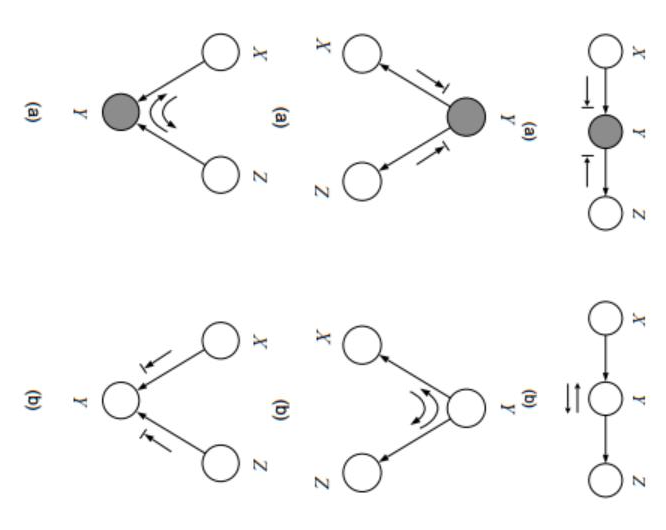
\includegraphics[width=.13\textwidth]{bayesball.png}
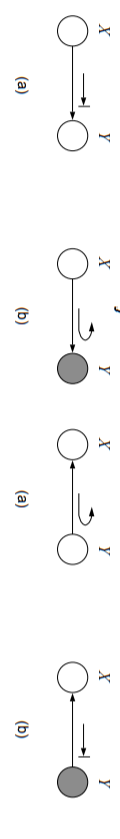
\includegraphics[height=.15\textwidth]{boundary.png}

\color[HTML]{6e2391}
\section{Learning} Want to use Bayes nets w/ real life data to get
vals. \textbf{Build models} of world from data
\paragraph{Learning in Bayes Nets} Given data in form of instances,
yes/no ans for all params of model. \textbf{Parameter estimation} w/
complete data: given Bayes struct $G$, choice of rep for CPDs
($P(X_i|Par(X_i))$). Goal to \colorbox{yellow}{learn CPD} of each node. \textbf{Assume
  all vars bin}. Assume instances $x_i, \ldots, x_m$ are
iid (\textbf{important}). \textbf{Learning prob} find set $\theta$ of
params s.t. data can be summarized by $P(x_j | \theta)$, $\theta$
depends on prob dist, i.e. just params of prob dist. More
\textbf{samples} the more you can trust data.
\paragraph{Goodness of param set} Depends on likelihood to gen obs
data. $D$ is data set. \textbf{Likelihood} of $\theta$ given $D$ is:
$L(\theta | D) = P(D | \theta)=P(x_1,\ldots,x_m)$ if iid
$=\prod_{i=1}^{m}P(x_i | \theta)$. \textbf{Sufficient statistic} of
data is func of data that summarizes enough info to compute
likelihood, i.e. $s(D)=s(D') \implies L(\theta|D)=L(\theta|D')$
\paragraph{Maximum Likelihood Estimation (MLE)}Choose params to
\textbf{maximize} likelihood. Instead of maxing prods, we can take
logs and max sum, since log is monotonic. $\log L(\theta|D) =
\sum_{i=1}^m \log P(x_i | \theta)$. \textbf{Derive} \& set to $0$ to
get max. For bern: $L(\theta|D)=\theta^{N(H)}(1-\theta)^{N(T)}, \log
L(\theta|D)=N(H)\log \theta + N(T)\log (1-\theta)$ derive $\to \theta
= \frac{N(H)}{N(H)+N(T)}$. With $k$ outcomes, $\theta = \frac{N_i}{N}$
Ex. $P(L|A)=\frac{P(L,A)}{P(A)}=\frac{\# l=1,a=1}{\# a=1}$
\paragraph{Param est in Bayes Net} Given instances, we are trying to
estimate prob of each node.
\\ \colorbox{red}{Problem} zero probs. For probs w/ lots of vars,
possible not all possible vars are seen in data, esp if rare. If val
not seen, MLE is $0$. To get around this, use \textbf{Laplace
  smoothing} for coin toss, instead of $\theta=\frac{N(H)}{N(H)+N(T)}$
use $\frac{N(H)+1}{N(H)+N(T)+2}$. If not Bernoulli, change $+2$ to
$+k$ in den and $+1$ for each outcome in num. Bad to use Laplace if
lots of params, will need a lot of data.
\\ To get MLEs of Berns in Bayes net given table, if uncond, get
proportion of true over total data. If cond, look at rows where
conditions are true (or false if we want given not $C$) and get
proportion.
\paragraph{Missing vals} Given data, some yes/no ans are
missing/undefined. \colorbox{red}{Problem} val missing might indicate
val, i.e. no x-ray could mean no bone problems. Can we use MLE? Can
throw out samples missing data, but biasing and bad. Otherwise we can
\textbf{consider both vals} of missing val, get diff likelihood for
both. Overall likelihood combines both. \colorbox{red}{Complicated}
given many missing vals!
\\ Can \colorbox{red}{no longer} est params locally \& indep like
complete data, we now have many local max (maxing likelihood is now
non-linear opt, w/ complete we have unique max) and no closed form
soln (complete has closed w/ assumptions)
\\ Assume prob of $X_i$ missing is indep its own val given observed
data. \colorbox{green}{2 solns} \textbf{Gradient ascent} Use hill
climbing to search through params, follow gradient of
likelihood. \colorbox{green}{Good} bc flexible for CPD forms, easy to
comp gradient, closely related to other learning, but
\colorbox{red}{bad} since soln needs to be in space of legal params to
ensure we get prob dists, sensitive to params/learning rate,
\textbf{slow}
\\ \textbf{Expectation Maximization} use current params to mk local
approx of likelihood that is nice. \textbf{Assume} underlying
dist.
\paragraph{EM} \textbf{Init} start with initial params (either
randomize or est from complete data instances). \textbf{Repeat}
\colorbox{yellow}{E-step}, complete data by assign vals to missing
based on curr
params(use probs to get expected prob of missing = x). \colorbox{yellow}{M-step}, compute MLE. \textbf{Convergence}
No change in E \& M step inbetween 2 consec iter
\\ \textbf{Hard EM} for each missing data, assign val most likely
(easier), \textbf{Soft EM} for missing, put weight on each val = prob,
use weights as counts (more common). \textbf{Comparison} soft does not
commit to vals for missing items. Considers all vals, better. But soft
requires comp cond probs, hard only requires comp most probable
\\ \textbf{Properties} Likelihood guarant to improve/stay same(stop) w/ each
iter. Guar to conv to local opt of likelihood, need local search, rand
restarts/diff init params. 
\\ \paragraph{Unsupervised Learning} What if var is always missing?
Can still est MLE. Relying on dist. Using Gaussian:
$\frac{1}{\sigma\sqrt{2\pi}}e^{-\left(\frac{1}{2\sigma^2}\right)(y-\mu)^2}$
\paragraph{K-means clustering} Cluster instances into $K$ distinct
classes. Need to know $K$ in adv, assum dist for each
class. \textbf{K-means alg}: 1.Ask how many clusters, 2.guess $k$ centers
$\left\{\mu_1,\ldots,\mu_k\right\}$, assm $\sigma^2$ known, 3.asgn each
data pt to closest $\mu$, 4.each center finds centroid of its pts
(i.e. mv center). Repeat 3-4. Essentially maxs likelihood of data.
\\ User must specify val of $K$, not
always poss, can try for diff vals of $K$, other meths try to learn
$K$. Stop when label of data points/cluster centers stop changing a
lot. \textbf{K-means is just hard EM with Gaussian}, can get local
opt/diff results, run mult times. There is also
soft EM vers of K-means, center calc with weights.
\\ $O(nkd)$, $k=\#centers, n=\#data,d=dim\ data$. Local opt. rand restarts to get better local opt, alternatively, choose
init centers, place $\mu_1$ on top of random data pt, $\mu_2$ on pt
furthest from $\mu_1$, $\mu_3$ on pt furthest from $\mu_1$ \& $\mu_2$
\paragraph{Supervised learning} Machine learning. \textbf{General
  learning prob}: Labeled examples $\langle
x_1,x_2,\ldots,x_3,y\rangle$, $x_j$ are \textbf{input vars/features/attribs},$y$
\textbf{desired output/output vars/targets}. Want learn func $h: X_1 \times X_2
\times \ldots X_n \to Y$, maps input to
output. Often \colorbox{yellow}{classification} prob, learn func for
categorical out. Else \colorbox{yellow}{regression}, out is
\textbf{continuous}. \textbf{Data set} = training
examples/instances. Training ex $i$ = $<x_{i,1},\ldots,x_{i,n},y_i>$,
$n$ attribs. $x_i$ is col vec with $x_{i,1},\ldots,x_{i,n}$. Training
set has $m$ ex. $X = X_1 \times \ldots \times X_n$ = space of input
vals, $Y$ = space of output vals.
\\ Dataset $D=X \times Y$, find func $h:X \to Y$ s.t. $h(x)$ good pred
for $y$, $h$ = \textbf{hypothesis}
\\ \textbf{Steps} decide input-output pairs, how to encode in/out,
class of hypotheses, error func, alg to search
\paragraph{Linear Hypothesis}
$Y$ is linear func of $X$: $f_W(x)=\sum_{j=0:m}w_jx_j$, $x_0=1$(no x,
this is intercept), $w_j$
are params/weights, $m=dim$ of obs space/\# features
\paragraph{Least-Squares} Min $\sum_{i=1}^n (y_i-w^Tx_i)^2$, use calc
to get soln or gradient descent if not possible. $f_W(X)=Xw,
Err(w)=(Y-Xw)^T(Y-Xw)$, minimize w/
$\frac{\partial{Err(w)}}{\partial{w}}=-2X^T (Y-Xw)$, $m$ eq (set to 0)
w/ $m$ unknowns. $X^T(Y-Xw)=0$
\\ $\hat{w}=(X^TX)^{-1}X^TY$, $\hat{Y}=X\hat{w}$. To pred new data,
$Y'=X'\hat{w}$ Cost: $nmp$ ops for mat mult, $m^3$ for inv, polytime
\colorbox{yellow}{$O(n^3)$}.
\paragraph{Polynomial fits} $y=w_0+w_1x+w_2x^2$, don't change method,
just more inputs, $x^2$ is a new feature, still linear in
weights. High deg \colorbox{red}{bad}, \textbf{overfitting}, hyp
explains too perfectly, does not \textbf{generalize} well. Use
\textbf{validation set} (from data) to est true error to pick best deg
\paragraph{Connectionist models} Comp architecture similar to brain
could dup some abilities. \textbf{Artificial Neural
  Networks}. Many neuron-like threshold switching units. Weighted
intercon among units. Parallel. Tune weights automat
\\ \textbf{Sigmoid func} $\sigma(z)=\frac{1}{1+e^{-z}}$,
squash to $1$, which neurons are
on. $\frac{d{\sigma(z)}}{d{z}}=\sigma(z)(1-\sigma(z))$. Neurons w/
sigmoid, input layer, output layer, hidden layers.
\\ \textbf{Feed-forward neural nets} $w_{ji}$ = weight on conn $i \to
j$. $x_{j0}=1 \forall j$ $o_j = \sigma(w_j \cdot x_j)$ output of unit
$j$, $w_j$ vec of weights entering $j$,
$x_j$ vec of inp to $j$, $x_{ji}=o_i$. To compute w/ NN, go through
network from inputs to output neurons passing signals through
activation funcs. Learn good weights. Need obj func (mean squared err),
learning alg, popular is \textbf{gradient
  descent}. $w^{k+1}=w^{k}-\alpha_k \nabla f (w^k)$, $\alpha_k>0$ step
size/learning rate for iter $k$,
$f(w^1)>f(w^2)>\ldots$, $lim_{k \to \infty}w^k = w$ local opt
\\ Overfitting (high valid err vs training err) comes from too many weights, train too long, weights
too extreme

\color[HTML]{2A2C5A}
\section{Temporal Inference}
Model change over time. $X_t$ \textbf{unobservable} vars @ time
$t$. $E_t$ \textbf{observable} ev vars @ $t$. Assume discrete time,
same struct @ ea timestep. $X_{t:t+k}=X_t ,\ldots,X_{t+k}$. Change
over time = \textbf{transition model} $P(X_t|X_{0:t-1})$ (prob of
being at $X=x$ at time $t$ given all other states from $0$ to $t-1$),
\textbf{sensor model} $P(E_t | X_{0:t}, E_{0:t-1})$
\\ \textbf{Markov Processes/Chains} Assumption $X_t$ depends on
bounded subset of $X_{0:t-1}$. \textbf{First-order Markov Process}
$P(X_t|X_{0:t-1})=P(X_t | X_{t-1})$. \textbf{Second-order}
$P(X_t|X_{0:t-1})=P(X_t|X_{t-2},X_{t-1})$. \textbf{Stationary process
  assump} Trans + sensor models \colorbox{yellow}{fixed} $\forall$ time steps, same cond
prob dists $P(X_t|X_{t-1})=P(X_{t+1}|X_t)$
\paragraph{Dynamic Bayesian Network} Bayes Net whose structure is
copied over time, dependencies between vars in neighbor time steps
\\ \textbf{Inf tasks} \textbf{Filtering} $P(X_t|e_{1:t})$,
\textbf{Prediction} $P(X_{t+k}|e_{1:t}), k>0$, \textbf{Smoothing}
$P(X_k|e_{1:t}), k<t$, \textbf{Most likely expl}
$argmax_{X_{1:t}}P(X_{1:t}|e_{1:t})$. 1st 3 tasks can use forward alg,
backward alg. Most likely can use Viterbi alg
\paragraph{Hidden Markov Model} 1 state + 1 sensor var / time
step. $P(X,E) = P(X_1)
\prod_{t=1}^{T-1}P(X_{t+1}|X_t)\prod_{t=1}^{T}P(E_t|X_t)$ where terms
after eq
are init state prob, state transition prob, emission prob. $N$
possible states, $W$ possible obs. $N$ init dist for $X_1$, $N^2$
trans dist, $NW$ emission dist. Use \colorbox{yellow}{MLE}. Init probs
$\pi_1, \ldots, \pi_N$ for $X_1$. Trans probs for $X_t \to X_{t+1},
A=\left\{a_{ij}\right\}, i,j\in[1,N]$. Emission probs $X_t \to E_t,
B=\left\{b_i(w_k),i\in [1,N], k\in[1,W]\right\}$
\paragraph{Forward alg} Efficiently marginalize all state seq using
dyn prog $P(E|\theta) = \sum_X P(E,X|\theta)$. \textbf{Trellis} of
possible state seq, col head is $E_i$, row head is $X_i$. Entries are
$\alpha_i(t)=P(E_{1:t,X_t = i | \theta})$. First get $\alpha_j(1)=\pi_j b_j(E_1)$ to fill first
col, then use prev col to fill next one w/ recur $\alpha_j(t)=\sum_{i=1}^N
\alpha_i(t-1)a_{ij}b_jE(t)$. Sum last col $P(E|\theta) =
\sum_{j=1}^N \alpha_j(T)$. $O(N^2T)$ for overall likelihood of seq.
\textbf{filtering}, rewrite goal as $P(X_t = i |
E_{1:t},\theta)=\frac{P(X_t=i,E_{1:t}|\theta)}{P(E_{1:t}|\theta)}$,
nume is $\alpha_i(t)$, den is from alg. \textbf{Prediction} Do
filtering for time $1$ to $t$ for $P(X_t|E_{1:t})$ then for $m=0:k-1$
$P(X_{t+m+1}|E_{1:t})=\sum_j
P(X_{t+m+1}|X_{t+m}=j)P(X_{t+m}=j|E_{1:t})$ save computations
$P(X_{t+m+1}|E_{1:t})$ for next iter
\paragraph{Backward alg} New trellis with cells $\beta_i(t) =
P(E_{t+1:T}|X_t = i, \theta)$. Prob of all prev emissions given curr
state is $i$. Excludes prob of curr emis. Start at $T$, $B_i(T)=1$. Then
$\beta_i(t)=\sum_{j=1}^Na_{ij}b_j(E_{t+1})\beta_j(t+1)$,
$P(E|\theta)=\sum_{i=1}^N \pi_i b_i (E_1)\beta_i (1)$,
\colorbox{yellow}{$O(N^2T)$}. Use for \textbf{smoothing},
$\alpha_i(k)=P(E_{1:k},X_k=i|\theta), \beta_i(k)=P(E_{k+1:t}|X_k = i,
\theta) \implies \alpha_i(k)\beta_i(k)=P(E_{1:t},X_k=i|\theta)$,
compute $P(X_{k}|E_{1:t})$ usind cond prob and $P(E_{1:t})$ (from
forward alg)
\paragraph{Work in Log Domain} Lots of mult, \colorbox{red}{avoid
  underflow} $\log \prod_{i=1}^{n} p_i = \sum_{i=1}^n \log p_i =
\sum_{i=1}^n a_i \implies \log \sum_{i=1}^n p_i = \log \sum_{i=1}^n
e^{a_i}=\log e^b \sum_{i=1}^n e^{a_i-b}=b+\log \sum_{i=1}^n e^{a_i-b}$
where $b=\max \ a_i$.
\\ \textbf{Sequence labelling} Viterbi, use forward alg but replace
sum with max. $X^* = arg\max_X P(X,E|\theta)=arg\max_XP(X|E,\theta)$,
$\delta_i(t)=\max_{X_{1:t-1}}P(X_{1:t-1},E_{1:t},X_t = i |
\theta)$. Alg: $\delta_j(1)=\pi_jb_j(E_1)$, then
$\delta_j(t)=\max_i\delta_i(t-1)a_{ij}b_{j}(E_t)$. Take $\max_i
\delta_i(T)$ \colorbox{yellow}{$O(N^2T)$}
\textbf{Backpointers} keep track of where ea max entry is,
work backwards to get best label seq 
\paragraph{Unsupervised TI} No state seqs, guess them, init params
rand, use Viterbi \colorbox{yellow}{EM}. Pred cur state seq using cur
model w/ Viterbi, then update cur params w/ cur pred \& repeat
\paragraph{Baum-Welch/Forward-backward alg} EM to HMMs. \textbf{E}:
expected cts for hidden structs w/ $\theta^k$, \textbf{M}: Get
$\theta^{k+1}$ to max likel
\\ Call req distribution for soft em in Baum as
\textbf{responsibilities}, $\gamma_i(t) = P(X_t = i | E,
\theta^k)=\frac{P(X_t = i, E |
  \theta^k)}{P(E|\theta^k)}=\frac{\alpha_i(t)\beta_i(t)}{P(E|\theta^k)}$
prob of being in state $i$ @ $t$ given obs seq under cur model,$
\xi_{ij}(t)=P(X_t=i,X_{t+1}=j|E,\theta^k)=\frac{P(X_t = i, X_{t+1}=j,
  E|\theta^k)}{P(E|\theta^k)}=\frac{\alpha_i(t)a_{ij}b_j(E_{t+1})\beta_j(t+1)}{P(E|\theta^k)}$
prob of trans from $i$ @ $t$ to $j$ @ $t+1$
\\ \textbf{Soft} MLE updates: $\pi_i^{k+1}=\gamma_i(1),
a_{ij}^{k+1}=\frac{\sum_{t=1}^{T-1}\xi_{ji}(t)}{\sum_{t=1}^{T-1}\gamma_i(t)},b_i^{k+1}(e_k)=\frac{\sum_{t=1}^T\gamma_i(t)|E_t
  = e_k}{\sum_{t=1}^T \gamma_i (t)}$
\\ Stop EM when training set likeli stops improv or prediction perf on
held-out development or validation set stops improv
\paragraph{Kalman Filtering}
HMMs with \textbf{continuous} state space
\\ \textbf{Linear Gaussian trans}: Assumed by Kalman, $P(X_{t+\Delta} =
x_{t+\Delta}|X_t = x_t, X_t' = x_t') = N(x_t +
x_t'\Delta,\sigma^2)(x_{t+\Delta})$. i.e. next pos is linear func of
current pos + \textbf{Gaussian noise}
\\ \textbf{One-step pred}
$P(X_{t+1}|e_{1:t})=\int_{x_t}P(X_{t+1}|x_t)P(x_t|e_{1:t})dx_t$
\\ \textbf{Filtering} $P(X_{t+1}|e_{1:t+1})=\alpha P(e_{t+1}|X_{t+1})P(X_{t+1}|e_{1:t})$
\\ \colorbox{red}{Limitations} Cant be used if nonlinear trans
model. Assume belief state = Gaussian
\paragraph{Particle filtering} Use samples of poss states to approx
belief. Pops of samples (particles) track high-likelihood. Replicate
particles proportional to likelihood for $e_t$.
\\ Assume belief @ t $N(x_t|e_{1:t})/N = P(x_t | e_{1:t})$. Propagate:
$N(x_{t+1}|e_{1:t})=\sum_{X_t}P(x_{t+1}|x_t)N(x_t|e_{1:t})$. Weight by
likeli
$W(x_{t+1}|e_{1:t+1})=P(e_{t+1}|x_{t+1})N(x_{t+1}|e_{1:t})$. Resample:
$N(x_{t+1}|e_{1:t+1})/N =\alpha W(x_{t+1}|e_{1:t+1})
=P(x_{t+1}|e_{1:t+1})$
\\ Easy for contin space, easy to implement, good for many dist,
increase \# particles for precision (Time/space complex grow
linearly w/ incr), hard to track rare
\paragraph{Speech Recognition} Probs: Noise, ambiguities,
co-articulation, intonation, accents, time. $P(Words|Signal) = \eta
P(Signal|Words)P(Words)$, where $Signal|Words$ is acoustic HMM (words
are hidden state vars, signal is ev vars) and
$Words$ is lang mod. English has 50 phones (distinct speech sounds),
make word pronunciation model, each state has onset/mid/end state for
each phone. HMM: Training via Baum-Welch + cont speech
signals. Recognition: use Viterbi for most likely seq of states ->
words. MLE: $P(w_i)=\frac{\# w_i}{N}, P(w_i|w_{i-1})=\frac{\#
  (w_{i-1},w_i)}{\# w_{i-1}}$

\color[HTML]{0450FB}
\section{Utility Theory}
Decision theory = prob theory + util theory.
What an agent wants. Need to be \textbf{actors}, choose actions in
rational way. Actions have consequences, want to max utility of acts.
\paragraph{Consequences} of an act are
\textbf{payoffs}/\textbf{rewards}. A rational method = eval benefit of
consq \& weigh by prob. To compare need: \textbf{set of consequences}
$C_a = \left\{c_1,\ldots,c_m\right\}$, \textbf{prob dist over cons}
$P_a(c_i), \sum_i P_a (c_i)=1$. A pair $L_a = (C_a, P_a)=[A,p; B, (1-p)]$ =
\textbf{lottery}. Pref: $A>B$ (A pref to B), $A\sim B$ (indiff), $A
\gtrsim$ (B \underline{not} pref to A)
\paragraph{Axioms of util theory}
\textbf{Orderability}: Linearity $(A>B)\lor (B>A) \lor (A \sim
B)$. Transitivity $(A>B)\land (B>C) \implies
(A>C)$. \textbf{Continuity} If $A>B>C, \exists $ lottery $L$ w/ $A$,
$C$ equiv to getting $B$, $\exists p, L = [p,A;(1-p) C]\sim
B$. \textbf{Substitutability} Add same prize w/ same prob to two equiv
lotteries, doesnt change pref. \textbf{Monotonicity} If 2 lots have
same prize, 1 giving best prize often pref. \textbf{Reduction of
  compound lotteries} 2 consecut lots $\to$ 1 equiv lot
\\ If we neglect an axiom, can show \colorbox{red}{not rational}
\paragraph{Utilities} map outcomes/states to vals, func
non-unique. Behaviour invariant wrt additive linear trans. W/
deterministic prizes only, only ordinal util (total order on prizes)
matter. Util don't need to obey same things as expec vals. Util models
should \colorbox{yellow}{capture risk attitude}, \textbf{risk neutral}
(util = expec), \textbf{risk averse} (util $<$ expec, rate of change slower) \textbf{risk
  seeking} (util $>$ expec, faster rate of change).
\\ Decision-theory \textbf{normative}, describ how rational agents
should act. Ppl \colorbox{red}{violate} axioms of util th. Ppl mk
diff decision based on how choices are \colorbox{yellow}{portrayed}
\paragraph{MEU} Choose act $\to$ maximize expected util
$\exists U$ s.t. $A \gtrsim B \iff U(A)\geq U(B),
U([p_1,C_1;\ldots;p_n,c_n]) = \sum_i p_i U(C_i)$. \textbf{Util func}
$U(x)$, \textbf{Expec Util} $EU(a | x) = \sum P(Eff(a)|x)U(Eff(a))$,
\textbf{MEU} $\max_a EU(a|x)$, \textbf{Optimal Action} $arg,\max_a
EU(a|x)$, \textbf{Policy} $\pi(x): X \to A$, pick action in all states
\paragraph{Decision Graphs} RVs are oval nodes, decisions/acts =
rectangles (no incoming arcs), utils = diamonds (no out-going
arcs). Compute opt act as \textbf{inference}
\paragraph{Information gathering} Env w/ hidden info, agent can choose
to do info-gath acts. Is it worth getting new info? \textbf{Value of
  info} specs util of evid that can be obtained. W/o risk, expec of
info = expec of best act w/ info $-$ expec val of best act w/o info
\paragraph{Val of Perfect info (VPI)} Hv evid $E$, best act $a^*$ w/
outcomes $c_i$. $EU(a^*|E) = \max_a U(A) = \max_a \sum_i
U(c_i)P(c_i|E,a)$. If we know $X=x$ then choose $a_x^*$: $EU(a^*_x|E, X=x) = \max_a U(A) = \max_a \sum_i
U(c_i)P(c_i|E,a, X=x)$. $VPI_E(X) = \sum_x P(X=x|E)EU(a^*_x|E,X=x) -
EU(a^*|E)$ 
\\ Props: \textbf{Non-negative} $\forall X,E VPI_E(X)\geq$, new info
\colorbox{green}{can't hurt}. \textbf{Non-additive} $VPI_E(X,X) \neq
2VPI_E(X)$, same info 2x doesn't benefit. \textbf{Order-indep}
$VPI_E(X,Y) = VPI_E(X)+VPI_{E,X}(Y) = VPI_E(Y) + VPI_{E,Y}(X)$
\\ \colorbox{red}{Don't always} want MEU, env may change/not fully
known. \textbf{Random choice models} choose act w/ highest expec util,
but keep non-zero probs for others (like Monte
Carlo). \textbf{Minimizing regret} minimize loss between current
behavior and some standard behavior. \textbf{Preference Elicitation}
finding ppl's pref $\to$ utils.
\paragraph{Learning utils from data}~
\paragraph{Bandit problems} Model of decision making under
uncertainty, \textbf{bandit} = name of a slot mach. Env is
\colorbox{red}{unknown}, don't know lottery, want to learn expect util
of band. \textbf{k-armed bandit}, collection of $k$
\colorbox{yellow}{actions}, each w/ lottery. Each choice =
\textbf{play}. After each play $a_t$, mach gives reward $r_t$ from
distrib assoc w/ $a_t$. Val of act $a$ given by expec util
$Q^*(a)=E[r|a]$. Want to \colorbox{yellow}{choose arms} to max rew in
\underline{long run}. \textbf{Est val of act}
$Q_n(a)=\frac{r_1+r_2+\ldots+r_n}{n}$. By law of large numbers,
$\lim_{n\to\infty}Q_n(a)=Q^*(a)$. To incrementally est:
$Q_{n+1}(a)=Q_n(a)+ \left(\frac{r_{n+1}-Q_n(a)}{n+1}\right)$
\paragraph{Exploration-exploitation trade-off} \textbf{explore} to
find what is best (need some random), \textbf{exploit} knowledge,
greedy $a_t^* = argmax_a Q_t(a)$. Prob may be
\colorbox{red}{non-stationary}, can't use sample avg (prob changes
over time). \colorbox{yellow}{emph} most recent rewards. Use constant
step size $\alpha \in (0,1),Q_{n+1}(a)=Q_n(a)+\alpha(r_{n+1}-Q_n(a)),
Q_{n+1}(a)=(1-\alpha)^nQ_0(a)+\sum_{i=1:n+1}\alpha(1-\alpha)^{n-i-1}r_i$. If
stationary, reduce explor over time, if not, can \colorbox{red}{never
  stop} explor.
\paragraph{Strats}
\textbf{Greedy} pick best arm $a$ w/ best est of
$Q_n(a)$. \textbf{$\varepsilon$-greedy} $\varepsilon\in (0,1)$
(small). On ea play, prob $\varepsilon$ explr random arm,
$1-\varepsilon$ explt best est. Can make $\varepsilon$ depend on
time. \colorbox{green}{v simple}, but leads
\colorbox{red}{discontinuities}. $\varepsilon=0=$greedy, $\varepsilon$
low, conv slow, $\varepsilon$ high, big var. \textbf{Softmax} act
probs func of cur vals $Q_t(a)$. At time $t$, choose $a$ with
$P(a_t)=e^{Q_t(a)/\tau}$, norm prob s.t sum is 1, $\tau$ is temp, if
$\tau$ high, favors explor, if low exploit. \textbf{Optimistic
  initialization} Assume good if no knowl. Initi act vals higher than
possible $Q_0(a)=\infty$, always pick best, random tie
break. \textbf{Upper-confidence bounds} conf intervals $\sigma = \sqrt{E[(X-\mu)^2]}$,
to explore, add $\sigma$ to $Q_t(a)$. Pick
$a$ via $Q(a)+\sqrt{\frac{2\log n}{n(a)}}$, $n$ is total \# acts
picked, $n(a)$ \# $a$ was picked
\\ All algs conv in limit to correct vals given stationary. UCB
fastest conv wrt regret. Simpler strats perform better in practice if
finite training
\paragraph{Contextual bandits} Add vector of measurements $\vec{s}$
s.t. there is state. Act val depends on $Q(\vec{s},a)=w_a^T \vec{s}$

\color[HTML]{DF541E}
\section{Markov Decision Processes}
Sequential decision-making, 1 decision affects next 1.
\paragraph{Markov Chain} Set of states $S$, trans prob
$T(s,s')=P(s_{t+1}=s'|s_t=s)$, initial state dist
$P_0(s)=P(s_0=s)$. Hidden Markov models = Markov chains of latent vars
w/ obs.
\paragraph{Sequential decision-making} At each $t$, agent in
$s_t$. Chooses act $a_t$, receives reward $R_{t+1}$ and can obs
$s_{t+1}$, markov chains w/ acts + rew
\paragraph{MDPs} States $S$, acts $A$, trans model
$T(s,a,s')=P(s_{t+1}=s'|s_t=s,a_t=a)$, prob $s \to s'$ under
$a$. Reward func $R(s,a)$, discount factor $\gamma \in [0,1]$, usually
close to 1, future rew less than current rew, $1-\gamma$ chance agent
dies at ea time step or inflation. \textbf{Planning} want to max
long-term utility aka \textbf{return}. Long-term util:
\textbf{episodic tasks} $U_t = R_t + R_{t+1} + \ldots R_T$, $T$ is
time when terminal state. \textbf{Continuing tasks} may go on forever,
$U_t = R_t + \gamma R_{t+1} + \gamma^2 R_{t+2} + \ldots =
\sum_{k=0}^{\infty}\gamma^j R_{t+k}, \gamma < 1$. \textbf{Policies} how agent
should act. \textbf{Deterministic pol} $\pi(s)=a$, \textbf{stochastic
  policy} $\pi(s,a)=P(a_t=a|s_t=s)$. Fix policy, MDP $\to$ Markov
chain w/ rew
\paragraph{State val func} Val func of pol $\pi$ is $V^\pi : S \to
\mathbb{R}$. Val of $s$ under $\pi$ is expect return if agent starts
from $s$ and picks act accord to $\pi$. $V^\pi(s)=E_\pi [U_t|s_t =
s]$. \textbf{Policy iteration} alg to find opt pol by computing state
val funcs. 1. Start with init pol $\pi_0$. 2. Alt between: \textbf{pol
eval} compute val of each $s$, $V^{\pi_i}(s)$. \textbf{Pol
improvement} improve cur pol to get $\pi_{i+1}$
\paragraph{Bellman's eq}$V^\pi (s)=E_{\pi}[U_t|s_t =
s]=E_{\pi}[R_t+\gamma U_{t+1}|s_t=s]$ Determ pol: $V^{\pi}(s)=R(s,\pi(s))+\gamma
\sum_{s' \in S}T(s,\pi(s),s')V^\pi(s')$, stoch pol: $V^{\pi(s)} =
\sum_{a \in A}\pi(s,a) (R(s,a)+\gamma \sum_{s'\in
  S}T(s,a,s')V^\pi(s'))$ In matrix form: $V^\pi = R^\pi + \gamma T^\pi
V^\pi$, $V^\pi$ is vector w/ val of ea state under $\pi$, $R^\pi$ is
vec w/ $R(s,\pi(s))$, $T^\pi$ is matrix w/ $T(s,\pi(s),s')$, can
sometimes solve explicitly: $V^\pi = (I-\gamma T^\pi)^{-1}R^{\pi}$
\paragraph{Iterative pol eval} Start with init guess $V_0$, for ea
iter $k$, update val func for all $s$, $V_{k+1}(s)=R(s,\pi(s))+\gamma
\sum_{s' \in S}T(s,\pi(s),s')V_k(s')$. Stop when converges (max change
between 2 iter smaller than threshold).
\paragraph{Searching for good pol} $\pi > \pi'$ if $V^{\pi}(s)\geq
V^{\pi'}(s) \forall s \in S$. Use local search. To improve pol:
$R(s,a^*)+\gamma \sum_{s' \in S}T(s,a^*,s')V^{\pi}(s')>\sum_{a\in
  A}\pi(s,a)(R(s,a)+\gamma \sum_{s \in
  S}T(s,a,s')V^{\pi}(s'))=V^{\pi}(s)$. Set $\pi(s,a^*)=1$ to increase
val of $s$. \textbf{Pol iter} $\pi'(s)=argmax_{a\in A}R(s,a)+\gamma
\sum_{s'\in S}T(s,a,s')V^{\pi}(s')$. Alg: start w/ init pol $\pi_0$
(rand), repeat: comp $V^\pi$ w/ pol eval $O(S^3)$, comp $\pi'$ greedy wrt
$V^\pi$ $O(S^2A)$, terminate when $V^\pi = V^{\pi'}$ (at most
$|A|^{|S|}$ iter)
\paragraph{Generalized pol iter} combine pol eval + pol improv, can
update val of 1 state and immediately improv to save time.
\\ \textbf{opt val func} $V^*(s)=\max_{\pi}V^{\pi}(s)$, best val at
any state. \colorbox{yellow}{unique} for finite MDP. \textbf{Opt pol} $\pi^*$ achieves opt val func, \underline{may not be
unique}, can have inf, ex. stochastic
\\ \textbf{Bellman Optimality Eq for $V^*$} $V^*(s)=\max_{a\in
  A}E[R_t+\gamma V^*(S_{t+1})|s_t=s,a_t=a]=\max_{a \in A}R(s,a)+\gamma
\sum_{s' \in S}T(s,a,s')V^*(s')$. Then we can comp $\pi^*(s)=argmax_{a
\in A}R(s,a)+\gamma \sum_{s'\in S}T(s,a,s')V^*(s')$
\paragraph{Value Iter Alg} Iter on val instead of pol. Start with init
approx $V_0$, for each iter $V_k(s)=\max_{a\in A}R(s,a)+\gamma\sum_{s'
\in S}T(s,a,s')V_{k-1}(s')$. Stop when max val change is below
threshold. Converges in lim to $V^*$. VI and PI conv to same, VI much
\colorbox{green}{cheaper} but may take \colorbox{red}{more
  iter}. $O(S^2A)$ per iter, $O(SA)$ if few succ states, polynomial
iter in $\frac{1}{1-\gamma}$
\\MDP \colorbox{red}{limitations}: get opt pol is poly in \# states but
\# states usually \underline{huge}. Dyn prog can solve up to $10^7$
states. VI and PI \colorbox{yellow}{assume} model is known
(trans+rew), soln: \textbf{reinforcement learning}. State sometimes
not observable, soln: \textbf{POMDPs} not discussed
\paragraph{Function approx} For large prob or continuous state space:
$V_w(s)$ approxs true val func, opt params $w$. Pop soln is to use
\textbf{linear func} $V_w(s)=\sum_mw_m\phi_m(s)$, $\phi_m(s)$ are
basis features w/ info about state like eval in games. $w_m$ are
weights
\\ Train weights from data: $MDP \to$ sample states $\to$ VI (gives
$x$) $\to FA$ (gives $y$) $\to V_\phi^*$ (gives $w$)
\\ $MSE:E_w = \sum_i [y_i - \sum_m w_m \phi_m (x_i)]^2$
\\ soln: $w_m=(\sum_i \phi_m (x_i)\phi_m(x_i)^T)^{-1}(\sum_i \phi_m
(x_i)y_i)$, $w_m(t+1)=w_m(t)-\alpha_i \sum_i \nabla_w (E^i_w)E^i_w$.
\\ Good basis set is small \& fits val func well
\paragraph{Reinforcement learning} Do acts, get
rewards. \textbf{Model-based}: Have policy for getting data (ex. rand
explor). Observe many trans in env. Learn approx model for
$R(s,a),T(s,a,s')$, use max likelihood for probs, supervised learn for
rew. \textbf{Monte-Carlo}: Gen several trajectories according to some
$\pi$, compute $V^{\pi}(s)$ via avg of observed returns after $s$, keep running avg
$V_{n+1}(s)=V_{n}(s)+\frac{1}{n+1}(U_{n+1}(s)-V_{n}(s))$. Avoid
keeping track of \# visited $n$, use learning rate
$V(s_t)=V(s_t)+\alpha(U(s_t)-V(s_t))$. \textbf{Temporal-Difference}
\colorbox{green}{estimate} return, don't need
$U(s_t)$. $V(s_t)=V(s_t)+\alpha(r_t+\gamma V(s_{t+1})-V(s_t))$,
dynamic prog like poli iter. A lot more updates. Hybrid dyn prog +
monte carl. \underline{Alg}: init $V(s)=0 \forall s$, repeat \#
wanted: pick start $s$. Repeat for each $t$: choose $a$ from $\pi$ and
$s$. Do $a$, get $r$ and $s'$. Comp TD error
$\delta = r + \gamma V(s')-V(s)$. Update $V(s)=V(s)+\alpha_s
\delta$. $s=s'$. If $s'$ not terminal, repeat another time step $t$ \\
\colorbox{green}{No model} req, only needs
exp. \colorbox{green}{on-line} incremental learn, learn before final
outcome, less mem+peak comp, faster conv than MC. Eligibility traces, shout
$\delta_t$ backwards, with temporal distance $\gamma \lambda, \lambda
\in [0,1]$. TD-learning used to get vals for given $\pi$. Explore vs
exploit, can use $\varepsilon$-greedy.
\\ Can correct function approximator using update rule $r_{t+1}+\gamma
V(s_{t+1})$. \textbf{On-line Gradient Descent TD} Init weight vector
of func approx $\vec{w}$. Pick start $s$. Repeat for ea $t$: choose $a$
based off $\pi,s$. Take $a$, get $r$ and $s'$. Comp TD error $\delta =
r + \gamma V(s')-V(s)$. Update $\vec{w} = \vec{w}+\alpha \delta \nabla
V(s)$. $s=s'$. For lin func approx, gradient is input feature vec


\color{black}
\section{Misc \& Ex}
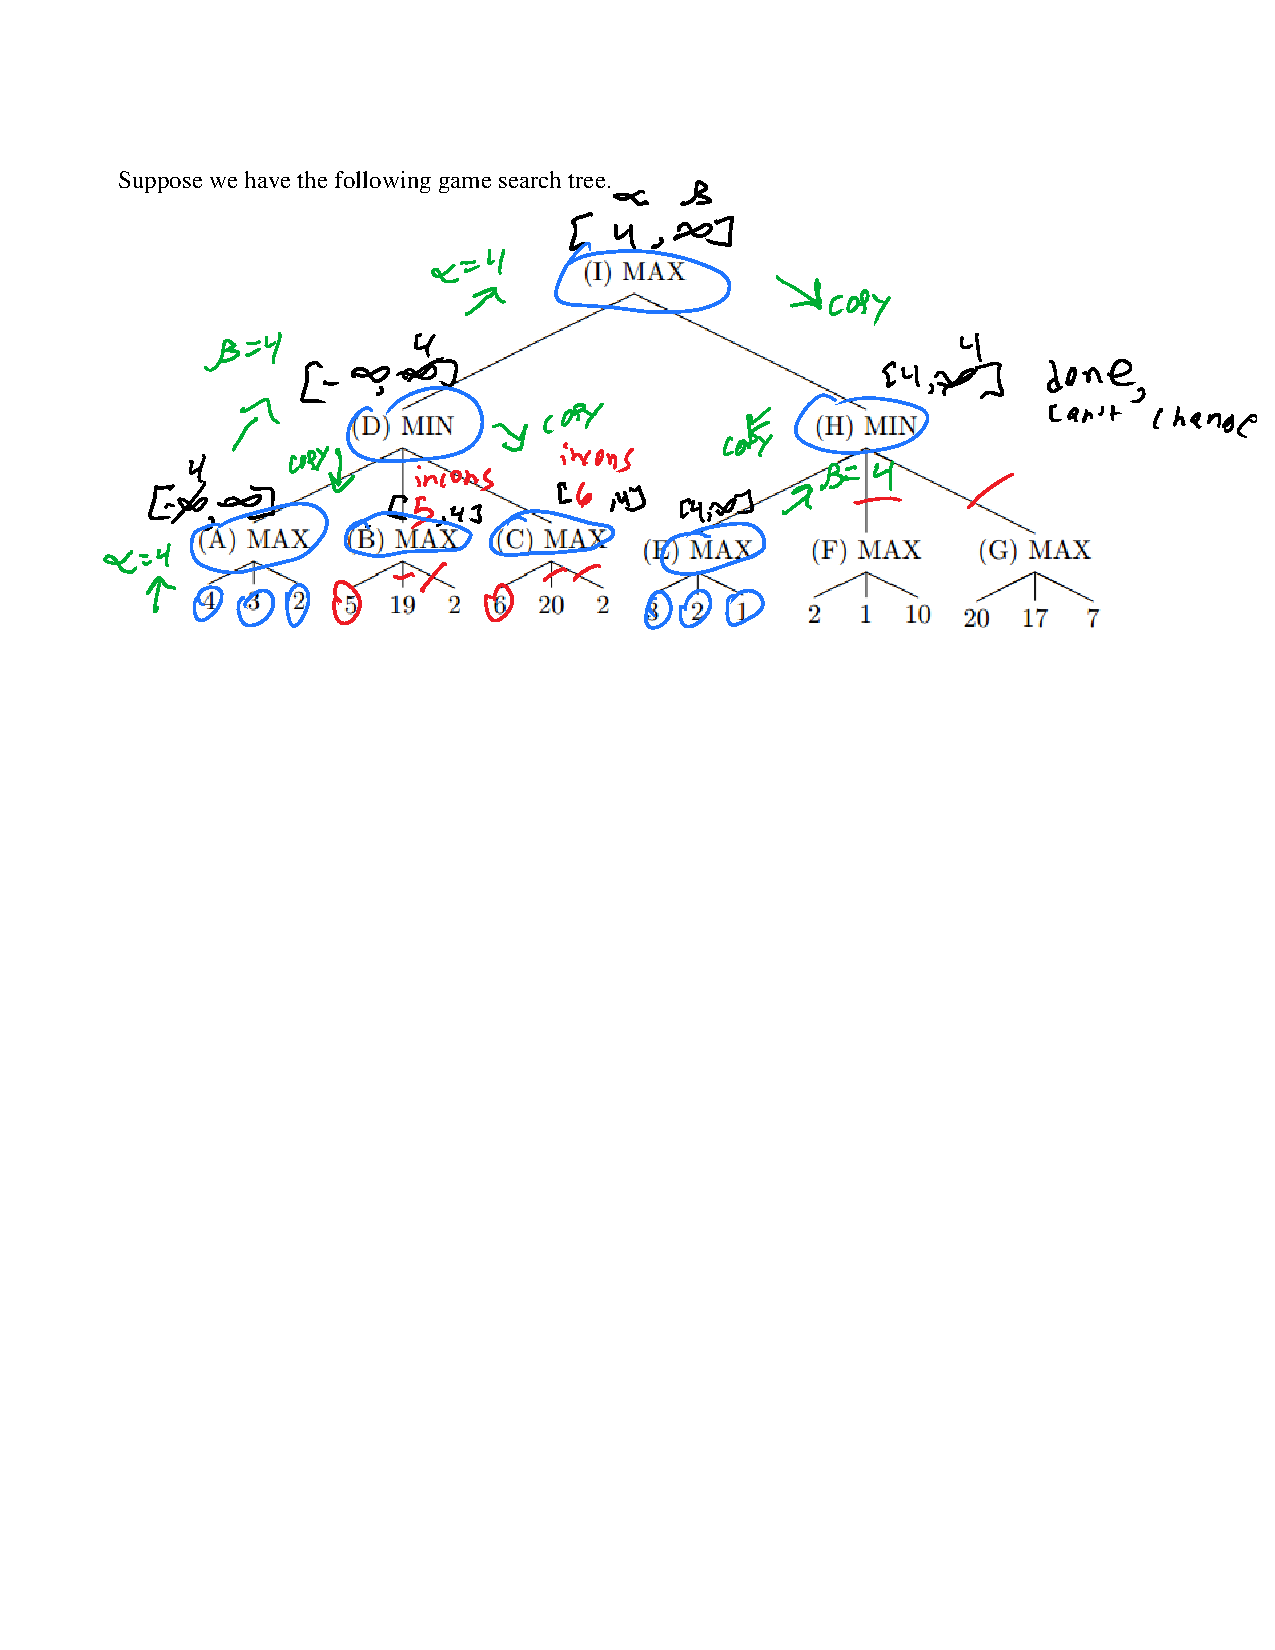
\includegraphics[width=.19\textwidth]{abprun.pdf}
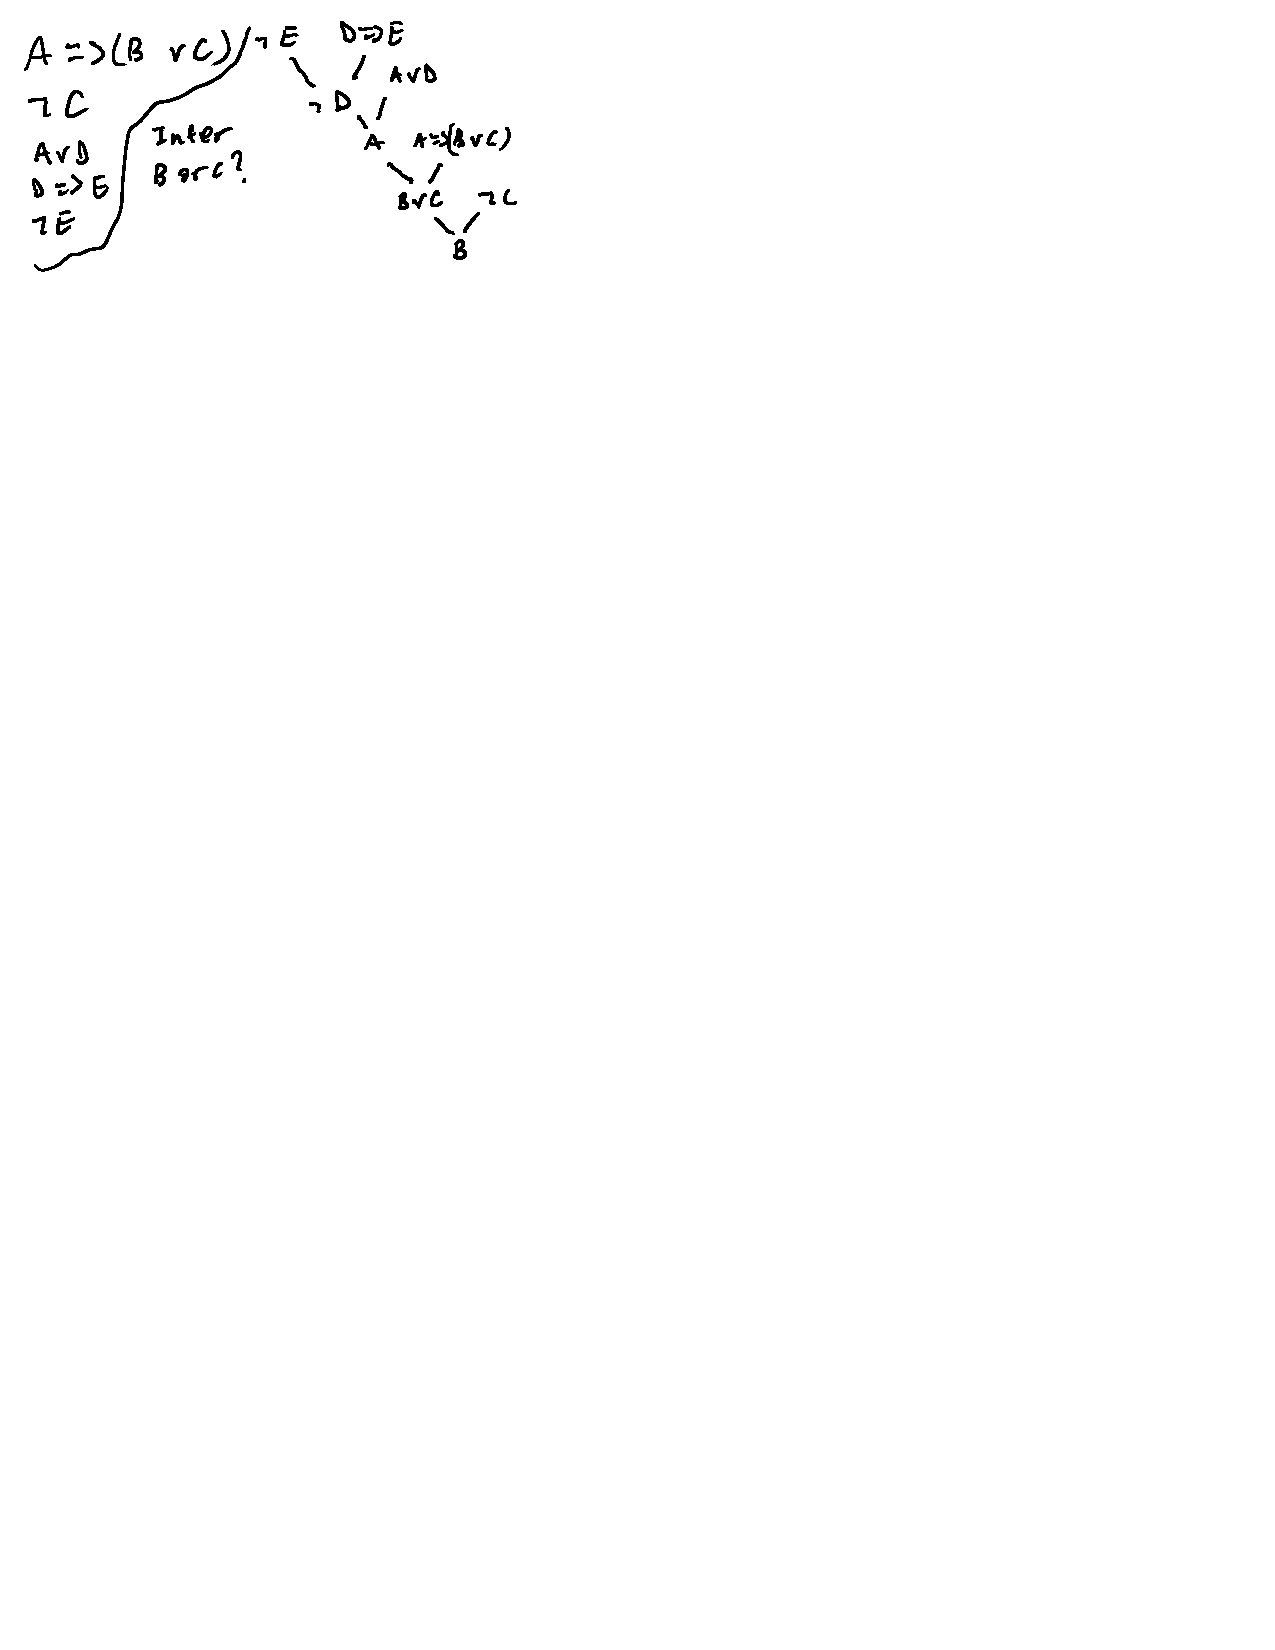
\includegraphics[width=.1\textwidth]{plinf.pdf}
\\ Local beam search with $k=1$ $\to$ hill climbing. LBS with 1 init
state and return as many as possible $\to$ BFS. SA with $T=0 \to $ HC,
SA with $T=\infty \to$ rand walk.
\\ Knapsack prob, var for each item, domain is $\{0,1\}$ (in bag or
not), constraint is sum should be less than cap.
\\ Map of diff cities, 2 friends in diff cities, each wait for other,
only 1 new node at a time. Want to meet. States: pair of cities. Succ:
neighbor nodes. Cost: max dist of both friends.
\\ Does it still make sense to use prob in deterministic world? Yes
might not be fully obs. Even w/ perf inf, might have long list to
reason about.

%%% Local Variables:
%%% mode: latex
%%% TeX-master: "Final"
%%% End:

\end{multicols*}
\end{document}